\documentclass[journal,article,submit,pdftex]{Definitions/mdpi}

\usepackage{tabularx}
\usepackage{caption}
\usepackage{enumitem}

\firstpage{1}
\setlength{\headheight}{20.0pt}
\makeatletter
\setcounter{page}{\@firstpage}
\makeatother

\pubvolume{1}
\issuenum{1}
\articlenumber{0}
\pubyear{2025}
\copyrightyear{2025}

\datereceived{}
\daterevised{} % Comment out if no revised date
\dateaccepted{}
\datepublished{}

\hreflink{https://www.mdpi.com/journal/iot} % If needed, change journal link

\Title{\texorpdfstring{IoT Retrofitting for a Remote Kinematics Laboratory in Engineering: Design, Implementation, and Technical Validation of a Prototype for the Study of UARM in a Hybrid Learning Environment}{Retrofitting IoT para laboratorio remoto de cinematica en ingenieria: diseno, implementacion y validacion tecnica de un prototipo para el estudio del MRUA en entorno hibrido de aprendizaje}}

\Author{Walter Santiago Sosa Mej\'ia}
\AuthorNames{Walter Santiago Sosa Mej\'ia}
\AuthorCitation{Sosa Mej\'ia, W.S.}

\address{%
\quad Pontificia Universidad Cat\'olica del Ecuador, Sede Esmeraldas; wssosa@pucese.edu.ec}

%-------------------------------------------------
% RESUMEN
%-------------------------------------------------

\abstract{Modernizing physics laboratories in resource-limited contexts poses significant challenges for higher education in Latin America, compounded by the need for hybrid and remote experimentation modalities. This article presents the design, implementation, and technical validation of a remote kinematics laboratory prototype for studying Uniformly Accelerated Rectilinear Motion (UARM), based on an IoT retrofitting strategy applied to pre-existing low-cost equipment. The proposed architecture integrates an ESP32 microcontroller as an Edge computing node, four infrared sensors, an MQTT broker on a Raspberry Pi~4, and a web interface built with Next.js/React for real-time control and visualization. To validate the system, 70 independent trials were conducted (35 remote and 35 in-person). Results demonstrate that the remote prototype achieves kinematic accuracy comparable to the traditional setup: mean differences between modalities are below 0.03~s at all four measurement points, standard deviations differ by less than 0.02~s ($\Delta\sigma < 0.02$~s), and the mean experimental acceleration is identical in both modalities ($\mu = 0.98$~m/s$^2$, with a theoretical expected value of $a \approx 0.92$~m/s$^2$). The Pearson correlation coefficients ($r = 0.61$--$0.62$) reflect the natural variability of the physical phenomenon rather than systematic biases. The successful event capture rate reached 98.5\% in remote mode. It is concluded that the IoT retrofitting methodology is a viable, scalable, and low-cost solution for democratizing access to quality experimental education in hybrid environments without requiring replacement of existing equipment.}

\keyword{Retrofitting; Internet of Things; Remote laboratories; MRUA; Low-cost instrumentation; Edge computing; Cloud services; Engineering education; Hybrid learning}

\begin{document}

%-------------------------------------------------
% INTRODUCCION
%-------------------------------------------------

\section{Introduction}

Physics laboratories are an essential component for the experimental verification of laws and models, as well as for the validation of measurement and control systems. Traditionally, these environments have operated on a strictly in-person basis, with analog or digital instrumentation requiring the physical presence of the user in the laboratory. However, the increasing digitalization of scientific infrastructure and the development of cyber-physical architectures have driven the design of platforms that enable remote and distributed operation, monitoring, and automation of experiments~\cite{r1}. The COVID-19 pandemic reinforced this trend by exposing the limitations of setups exclusively dependent on local presence, accelerating the adoption of remote laboratories and cloud-connected instrumentation systems~\cite{r2}.

In this context, a recurring problem becomes evident: many physics laboratories continue to rely on setups centered on in-person operation, with minimal automation, no remote access mechanisms, and difficulties in systematically recording and managing data. This situation is particularly notable in Latin America, where numerous laboratories operate with aging instrumentation and limited resources for equipment renewal or incorporation of advanced connectivity solutions~\cite{r3,r4}. The physics laboratory at the Pontificia Universidad Cat\'olica del Ecuador, Esmeraldas campus, is a representative example: it has toy-type tracks, low-friction carts, and conventional measurement elements for kinematics and dynamics experiments, but lacks automation capabilities and remote access. In this scenario, designing architectures that enable retrofitting of existing setups with low-cost IoT technologies becomes a technical and operational necessity.

\subsection{Related Work and Research Gap}

Recent literature evidences significant advances in the modernization of physics laboratories through digital technologies, particularly via remote and hybrid laboratories and IoT-based retrofitting strategies. Studies such as those by Lahme \textit{et al.}~\cite{r1} document the increasing use of microcontrollers, sensors, and digital platforms in laboratory courses, highlighting both their potential and the technical barriers associated with their adoption. Complementarily, works oriented toward the remote control of physical systems, such as those presented by Guerrero-Osuna \textit{et al.}~\cite{r4} and Fuertes \textit{et al.}~\cite{r3}, demonstrate the viability of integrating embedded hardware, cloud services, and web interfaces for operating real experiments with adequate response times.

In the specific context of retrofitting existing equipment, Viswanadh \textit{et al.}~\cite{r2} propose low-cost architectures that enable instrumenting pre-existing laboratory setups without structural modifications, while Lustig \textit{et al.}~\cite{r5} introduce modular platforms that decouple experimental hardware from access and visualization services. Zhao~\cite{r6} extensively reviews solutions based on mass-market sensors and video analysis, demonstrating that reasonable measurement quality can be obtained using accessible and widely available devices.

Nevertheless, despite these contributions, several limitations are identified in the existing literature. First, many works focus on the functional demonstration of remote platforms or usability evaluations, without delving into the quantitative validation of experimental fidelity against in-person reference setups. Second, there is a lack of studies that systematically analyze the technical performance of classic physics experiments such as kinematics when executed remotely, considering metrics such as detection time error, internal data coherence, and system stability. Finally, few studies address these issues in resource-limited contexts, where the reuse of existing equipment through retrofitting is particularly relevant.

In this framework, the present work differentiates itself by proposing and validating a hybrid physics laboratory model based on IoT retrofitting. To contextualize our contribution within modern IoT architectures, we adopt the layered approach proposed by Dizdarevic and Jukan~\cite{r7}, who highlight the importance of integrating Edge and Cloud computing capabilities to reduce latency in educational environments---a lesson we have applied through the use of the control device for edge processing. Furthermore, to ensure operational continuity and universal accessibility, we follow the principles of Azad~\cite{r8} on the deployment of IoT-based remote laboratories, guaranteeing system robustness against disconnections. Finally, the validation of our system aligns with the ``digital twins'' methodology described by Palmer \textit{et al.}~\cite{r9}, using direct comparison between physical sensor data (the ``real twin'') and the expected theoretical model, thereby ensuring rigorous quantitative verification.

More recently, Lustig \textit{et al.}~\cite{r10} propose an end-to-end retrofitting architecture based on ESP32, Raspberry Pi, and the MERN stack that enables remote access to optics experiments; their architectural approach is structurally analogous to the one proposed in this work, although it does not include quantitative validation of kinematic equivalence between modalities. Complementarily, P\'erez-Cham\'e \textit{et al.}~\cite{r11} develop a low-cost ESP32-based platform for fundamental physics in undergraduate engineering, demonstrating the viability of the selected hardware for resource-limited educational environments. In terms of real-time data acquisition, Marosan \textit{et al.}~\cite{r12} validate the use of ESP32 with the MQTT protocol for IoT applications with precise timing requirements, confirming the suitability of the control module adopted in this study. Similarly, Chang \textit{et al.}~\cite{r52} deployed an IoT-based remote platform for undergraduate mechanics labs, obtaining precision results comparable to those in this work and confirming the replicability of the approach across different institutional contexts.

Despite the advances described, the following gaps in the literature are identified: (1)~most works validate remote platforms in functional or usability terms but do not perform rigorous quantitative validation of measurement equivalence between remote and in-person modalities; (2)~very few studies analyze the technical performance of classic kinematics experiments executed remotely, considering metrics such as temporal error, data coherence, and experimental acceleration; (3)~few studies address these issues in the specific context of Latin American universities with limited resources~\cite{r13,r14}, where retrofitting is particularly pertinent. To the best of the authors' knowledge, no previous work quantitatively validates kinematic equivalence between remote and in-person modalities on low-cost equipment through IoT retrofitting in the context of resource-limited Latin American institutions.

\textit{\textbf{Research question:} Can a low-cost IoT retrofitting system on pre-existing equipment reproduce kinematic measurements of UARM with comparable accuracy and stability to an in-person reference setup, in a resource-limited university laboratory?}

The \textbf{general objective} of this work is to design, implement, and technically validate a remote laboratory prototype based on IoT retrofitting for the study of UARM. The specific objectives are: (1)~design a three-layer IoT architecture with Edge computing embedded in an ESP32 control module; (2)~implement the integrated hardware, firmware, backend, and web application system; (3)~quantitatively validate the equivalence between modalities through Pearson correlation analysis, velocity profiles, and acceleration distributions.

The main \textbf{contributions} of this work are:
\begin{itemize}
  \item Design and validation of a three-layer IoT architecture with Edge computing embedded in ESP32 for kinematics experiments in resource-limited environments.
  \item Quantitative validation of equivalence between remote and in-person modalities through 70 trials with Pearson correlation metrics ($r = 0.61$--$0.62$), experimental acceleration, and event capture rate (98.5\%).
  \item Demonstration that the natural variability of UARM explains the moderate correlation coefficients and does not constitute a systematic bias of the IoT system.
  \item Publication of open-source code on GitHub (RemotePhysicsLab~\cite{r15}) with complete documentation for replication in other laboratories.
\end{itemize}

The remainder of this article is structured as follows: Section~\ref{sec:metodos} describes the materials and methods; Section~3 presents the experimental results; Section~4 discusses the implications and compares with related works; finally, Section~5 presents the conclusions and future work directions.

%-------------------------------------------------
% MATERIALES Y METODOS
%-------------------------------------------------

\section{Materials and Methods}
\label{sec:metodos}

\subsection{Research Design}

The research was conceived as an applied technical study oriented toward the design, construction, and validation of a remotely controlled physics laboratory prototype using IoT technologies. A quantitative approach with a descriptive scope was adopted, as the central analysis variables correspond to measurable physical quantities (detection times, recorded events, fault occurrences) obtained from instrumental records of the system, which are subsequently described and compared without involving human participant groups. The methodological approach was aligned with the logic of Design Science Research (DSR), in which the central objective is to build a technological artifact and evaluate it systematically~\cite{r16}, and took as a general reference the system life cycle processes described in the ISO/IEC~15288 standard to organize the requirements, design, implementation, integration, and operation phases of the prototype~\cite{r17}.

Based on this framework, the scope of the present research was defined to focus on the technical evaluation of the uniformly accelerated rectilinear motion (UARM) experiment, specifically on the accuracy and consistency of the physical variables measured and calculated by the remote system compared to an equivalent in-person reference setup.

%-------------------------------------------------
\subsection{Hardware and Software Used}

To ensure a clear and replicable presentation, the materials used are grouped into two tables: hardware components (Table~1) and software tools (Table~2). Figure~1 summarizes how these elements are integrated into the overall system architecture.

\begin{table}[H]
	\caption{Hardware components of the IoT-based hybrid physics laboratory prototype.\label{tab:hardware}}
	\small
	\begin{adjustwidth}{-\extralength}{0cm}
		\renewcommand{\arraystretch}{1.5}
		\renewcommand{\tabularxcolumn}[1]{m{#1}}
		\begin{tabularx}{\fulllength}{>{\raggedright\arraybackslash}m{4.5cm}Xc}
			\toprule
			\textbf{Device Category} & \textbf{Consolidated Technical Specification} & \textbf{References} \\
			\midrule
			Mechanical Experimental System & Hot Wheels-type track\textsuperscript{\textregistered} used as a rectilinear motion rail with a low-friction cart adapted for kinematics experiments & \cite{r18,r19} \\
			Sensing and Data Acquisition System & Four infrared sensors for passage detection and time measurement & \cite{r20} \\
			IoT Control and Processing Unit & Control module DevKit (30 pins, USB-C, integrated WiFi and Bluetooth connectivity) & \cite{r21,r53} \\
			Mechanical Structure and Physical Support & 3D-printed supports, reinforcements, and mechanical assemblies for mounting sensors, actuators, and structural elements & \cite{r22,r23,r24,r25} \\
			Actuators and Motion Control & SG90 servo motor (180\textdegree), NEMA 17 bipolar stepper motor, and L298N H-bridge module for motion control & \cite{r26,r27,r28} \\
			Local User Interface & 20x4 LCD display with I\textsuperscript{2}C interface and mechanical push button for local interaction & \cite{r29,r30} \\
			Communication and Connectivity & IEEE 802.11 (WiFi) wireless standard, USB-C cable, and Dupont wires for electrical interconnection & \cite{r31,r32,r33} \\
			Power Supply and Protection System & AC--DC 12~V / 1~A adapter and plastic enclosure for electronics projects (135 $\times$ 75 $\times$ 40 mm) & \cite{r34,r35} \\
			Remote Visualization System & Insta360 Link webcam with 4K resolution and AI-assisted tracking features & \cite{r36} \\
			IoT System Server and Management & Raspberry Pi 4 Model B for communications management, storage, and system monitoring & \cite{r37} \\
			\bottomrule
		\end{tabularx}
	\end{adjustwidth}
\end{table}


\begin{table}[H]
	\caption{Software tools used in the IoT-based hybrid physics laboratory system.\label{tab:software}}
	\small
	\begin{adjustwidth}{-\extralength}{0cm}
		\renewcommand{\arraystretch}{1.5}
		\renewcommand{\tabularxcolumn}[1]{m{#1}}
		\begin{tabularx}{\fulllength}{>{\raggedright\arraybackslash}m{3.5cm}X>{\centering\arraybackslash}m{3.5cm}c}
			\toprule
			\textbf{System Layer} & \textbf{Software Tools} & \textbf{Versions} & \textbf{Referencias} \\
			\midrule
			IoT Communication & EMQX, MQTTX Desktop & 5.10.2; 1.12.1 & \cite{r38,r39} \\
			Backend and Services & Node.js (LTS), Express & 24.11.1; 5.1.0 & \cite{r40,r41} \\
			Data Persistence & MongoDB Server, MongoDB Driver, Mongoose & 8.2.2; 6.3.0; 8.5.1 & \cite{r42,r43} \\
			Frontend and Visualization & Next.js, React & 16.0; 19.2.0 & \cite{r44,r45} \\
			Embedded Development & Arduino IDE & 2.3.4 & \cite{r46} \\
			Languages and Support & Python & 3.14.1 & \cite{r47} \\
			\bottomrule
		\end{tabularx}
	\end{adjustwidth}
\end{table}

\subsection{Overall System Architecture}

The overall system architecture is organized into three well-differentiated layers~\cite{r48} (Figure~1). Layer~1 groups the perception elements of the experiment, including the UARM laboratory cart, the track, the four infrared sensors, the experiment camera, and the ESP32 control module with integrated WiFi connectivity~\cite{r21,r53}, which is responsible for acquiring sensor signals and transmitting them via MQTT over WiFi. Layer~2 corresponds to the local network and server, consisting of the WiFi router or access point and the Raspberry Pi, where the EMQX broker, video server, and web API that processes the data are executed. Finally, Layer~3 includes the web-based user interface, from which the instructor and student can visualize data tables and graphs of position, velocity, and acceleration, as well as observe the experiment video and send control commands to the system.
\begin{figure}[H]
\centering
\includegraphics[width=\textwidth]{figures/fig1_arquitectura_labfisica.png}
\caption{Three-layer architecture of the IoT-retrofitted physics laboratory. Diagram elaborated following the fundamental three-layer model~\cite{r48} with the Eraser tool~\cite{r49}.}
\label{fig:arquitectura}
\end{figure}

Figure~\ref{fig:arquitectura} illustrates the overall system architecture. Figure~\ref{fig:hardware_connection} shows the wiring diagram of the control module, detailing the connections between the ESP32 and the infrared sensors, servo motor, L298N driver, LCD display, and start button.

\begin{figure}[H]
\centering
\includegraphics[width=0.8\textwidth]{figures/Hardware connection diagram of the proposed prototype.png}
\caption{Control module wiring diagram. Image generated with the assistance of ChatGPT~\cite{r50}.}
\label{fig:hardware_connection}
\end{figure}

\paragraph{Edge Computing Processing.}
A central aspect of the proposed architecture is the implementation of Edge computing processing in Layer~1. The control module locally executes event detection through hardware interrupts and generates the timestamp of each event \textbf{before} its transmission via MQTT~\cite{r12}. This ensures that WiFi network latency---inherent to any distributed system---affects only the visualization in the web interface, without degrading the precision of the recorded physical timestamps. This design follows the model of Dizdarevic and Jukan~\cite{r7}, who highlight effective latency reduction through Edge computing in educational IoT environments, and is consistent with the principles of Hern\'andez \textit{et al.}~\cite{r51} for remote laboratories robust against disconnections.

Table~\ref{tab:connections} details the electrical connections and pin assignment of the ESP32 control module, specifying the signal type and power supply required by each prototype component.

\begin{table}[H]
	\caption{Detailed system connections and pin assignment of the control module.\label{tab:connections}}
	\small
	\begin{adjustwidth}{-\extralength}{0cm}
		\renewcommand{\arraystretch}{1.3}
		\renewcommand{\tabularxcolumn}[1]{m{#1}}
		\begin{tabularx}{\fulllength}{clXccc}
			\toprule
			\textbf{N\textsuperscript{o}} & \textbf{Component} & \textbf{Function in the Experiment} & \textbf{Control Mod. Pin} & \textbf{Signal Type} & \textbf{Power Supply} \\
			\midrule
			1  & Sensor S1      & Motion start detection         & GPIO 15 & Digital input (PULLUP) & 5 V / GND    \\
			2  & Sensor S2      & Intermediate section 1 detection            & GPIO 25 & Entrada digital (PULLUP) & 5 V / GND    \\
			3  & Sensor S3      & Intermediate section 2 detection            & GPIO 12 & Entrada digital (PULLUP) & 5 V / GND    \\
			4  & Sensor S4      & End of track detection           & GPIO 13 & Entrada digital (PULLUP) & 5 V / GND    \\
			5  & Manual button  & Experiment start / cancellation    & GPIO 18 & Entrada digital (PULLUP) & GND          \\
			6  & Servo motor    & Initial cart push / release & GPIO 5  & PWM                      & 5 V / GND    \\
			7  & L298N -- ENA   & Motor acceleration control (NUARM) & GPIO 14 & PWM                      & 5 V / GND    \\
			8  & L298N -- IN1   & DC motor direction                  & GPIO 27 & Digital output           & N/A          \\
			9  & L298N -- IN2   & Direcci\'on del motor DC                  & GPIO 26 & Salida digital           & N/A          \\
			10 & LCD 16$\times$2 -- SDA & I2C communication (data)       & GPIO 21 & I2C                      & 5 V / GND    \\
			11 & LCD 16$\times$2 -- SCL & I2C communication (clock)       & GPIO 22 & I2C                      & 5 V / GND    \\
			12 & Motor DC       & Accelerated motion generation     & L298N   & Power                 & 11--12 V     \\
			13 & Common ground  & System electrical reference        & GND     & N/A                      & Common       \\
			\bottomrule
		\end{tabularx}
	\end{adjustwidth}
\end{table}



\subsection{Population, Sample, and Experimental Environment}

This study does not involve a population of human subjects or organizational units, but rather an instrumented physical system whose behavior is evaluated from a technical perspective. For this reason, instead of defining a population and sample in the classical sense of quantitative research, this subsection focuses on describing the laboratory experimental environment and the way in which the trials performed on the setup were planned. In total, 70 trials were conducted, corresponding to 35 in-person tests and 35 remote tests.

The experiment was conducted in the physics laboratory of the Pontificia Universidad Cat\'olica del Ecuador, Esmeraldas campus, which has a leveled workbench, access to regulated electrical power, and local network connectivity through a WiFi access point. In this space, the Hot Wheels\textsuperscript{\textregistered}-type track~\cite{r18}, the low-friction laboratory cart~\cite{r19}, the four infrared sensors~\cite{r20}, the control module~\cite{r21,r53}, and the Insta360 Link camera~\cite{r36} were installed, forming the physical setup of the UARM experiment. The Raspberry~Pi~4 used as the IoT server~\cite{r37} was located in the same laboratory and connected to both the WiFi access point~\cite{r32} and the institutional wired network.

%-------------------------------------------------
\subsection{Implementation Procedure}

The procedure followed to develop and evaluate the prototype was organized into four stages, consistent with the specific objectives of the study: system design and definition of the IoT architecture for the remote laboratory, hardware and software implementation, experimental environment configuration with trial execution in remote and in-person modes, and technical validation of prototype operation.

First, a requirements gathering was conducted together with the instructor responsible for the Physics course, considered an expert in the UARM experiment. In this stage, the events that the system should record (cart passage through each sensor), the minimum information needed to describe the experiment, and the acceptable setup conditions in the laboratory were identified. Based on these inputs, the IoT architecture of the remote laboratory was defined, specifying hardware components, software services, and data flow between the ESP32, MQTT server, backend, and web application. Design decisions were documented in the README files of the public RemotePhysicsLab repository~\cite{r15}, in the \texttt{frontend} and \texttt{backend} folders.

In a second phase, the IoT prototype was implemented (Figure~1). The physical track setup was built and the infrared sensors were installed at fixed positions along the cart's path. The control module was programmed using the Arduino IDE environment to read sensor states and send MQTT messages with timestamps to the MQTT server deployed on the Raspberry Pi. In parallel, the experiment camera and video server were configured so that the signal could be consumed from the web browser. During this phase, unit tests were performed to verify correct sensor reading, WiFi connectivity, publication to defined MQTT topics, and continuous reception of the video signal. Subsequently, the experimental environment was configured and trial execution proceeded. The cart starting point, track inclination, and sensor positions were fixed, keeping these parameters constant across all tests. With this configuration, trial series were conducted in two modalities: on one hand, remote operation through the laboratory's web interface, where the user activated the experiment, observed the cart movement through near-real-time video, and detection times were automatically recorded in the system; on the other hand, in-person operation using a reference setup without the IoT component, which served as a baseline for comparing time measurements and derived kinematic quantities. In both modalities, the experiment was repeated multiple times to obtain a sufficient set of records. Finally, the technical validation of the prototype was performed. For this purpose, data generated by the remote system and the in-person setup were compiled, organizing them into comparative tables by sensor and by repetition. Based on these tables, the coincidence of detection times between both modalities was evaluated, it was verified whether the remote system recorded all expected events in each cart run, and incidents related to system stability were qualitatively documented, such as service outages, disconnections, or need for restart during testing sessions. This procedure allowed verifying the extent to which the prototype consistently reproduces the UARM experiment in remote mode compared to the in-person reference setup.

\begin{figure}[H]
\centering
\includegraphics[width=\textwidth]{figures/Experimental procedure flowchart.png}
\caption{Data flow during laboratory operation.
Infrared sensor readings associated with the cart passage are sent by the control module to the MQTT server via MQTT.
The backend processes the messages, records them in MongoDB, and exposes them to the web application, which in turn presents the data and experiment video to the user. Elaborated with the AI-assisted diagramming tool Eraser~\cite{r49}}
\label{fig:flujo-datos}
\end{figure}

%-------------------------------------------------
\subsection{Evaluation Metrics}

In the technical validation of the prototype, the analysis focuses on quantifying the degree of association and agreement between the measurements obtained in the in-person modality and those recorded by the IoT system. The objective is to determine whether the retrofitting-based technological instrumentation is capable of replicating the stability and precision of the traditional setup. To this end, an experimental campaign of 70 total trials was conducted, divided into 35 manual (in-person) records and 35 automated (remote) records.

As a fundamental performance metric, the Pearson correlation coefficient (\(r\)) is adopted, which allows evaluating the fidelity with which the remote laboratory reproduces the behavior observed in the physical reference setup. The coefficient is calculated for each of the four sensors (S1 to S4) independently. Since the trials in both modalities were performed as independent physical events, the analysis does not seek a point-by-point trial-to-trial correspondence, but rather to certify that both systems capture the dynamics of UARM consistently.

The correlation coefficient is defined by the following equation:

\begin{equation}
r = \frac{\sum_{i=1}^{n} (x_i - \bar{x})(y_i - \bar{y})}{\sqrt{\sum_{i=1}^{n} (x_i - \bar{x})^2} \sqrt{\sum_{i=1}^{n} (y_i - \bar{y})^2}}
\label{eq:pearson}
\end{equation}

Where \(x_i\) represents the times measured in the in-person modality (manual reference) and \(y_i\) the times measured in the remote (IoT) modality for a series of \(n=35\) trials per modality, with their respective means \(\bar{x}\) and \(\bar{y}\). A value of \(r\) close to 1 validates that the IoT instrumentation captures the natural variability of the kinematic phenomenon with fidelity equivalent to in-person timing.

It is important to note that, since the trials in both modalities were executed as independent and unpaired physical events, the Pearson coefficient does not measure point-to-point agreement between series, but rather the coincidence in capturing the dynamic variability of the phenomenon. For this reason, the analysis is complemented with the Bland--Altman method~\cite{bland1986}, which directly evaluates the limits of agreement between the measurements of both modalities~\cite{giavarina2015}.



%-------------------------------------------------

\subsection{Data Analysis Methods}

The data recorded by the IoT prototype (hybrid modality) and by the in-person reference setup were exported as structured text files containing the timestamps associated with the cart passage through each sensor and the configuration of each trial. These records were organized in spreadsheets and subsequently processed using scripts developed in Python~3.14.1~\cite{r47}.

The analysis focused on the consistency of passage times per sensor and on calculating the Pearson correlation between the hybrid and in-person modalities. Scatter plots were generated to visualize the proximity between the obtained measurements and detect possible prototype deviations. The numerical and graphical results are presented and discussed in the Results section. In a first stage, data from both modalities were integrated into comparative tables that group, by trial, the passage times recorded by the hybrid system and by the in-person setup. In a second stage, scatter plots and histograms were generated to visualize the proximity between the measurements obtained in both modalities and validate the consistency of the prototype through correlation analysis. The numerical results of these comparisons, as well as the tables and graphs derived from processing in Python~3.14.1~\cite{r47}, are presented and discussed in the Results section, where the agreement of the hybrid laboratory against the in-person reference setup is analyzed in detail.


%-------------------------------------------------
\subsection{Validity and Reliability Control}

The validity and reliability control focused on ensuring that the measurements taken by the IoT prototype were consistent with the expected physical behavior of the UARM experiment and comparable with those obtained in the in-person reference setup. First, measurement validity was verified through specific tests of cart detection by the infrared sensors. To this end, trial tests were conducted in which the cart moved in a controlled manner along the track, observing in real time the state of the control module's digital inputs and the messages published via MQTT. The height and orientation of each sensor were adjusted to ensure that the cart passage generated clean signal transitions (active/inactive) without spurious triggers from ambient noise or unwanted reflections. The track used has an effective length of 160~cm, over which the four detection sensors were distributed at intervals of 53.2~cm, providing well-defined distances for calculating velocities and accelerations from passage times.

Additionally, the measurement of fixed distances between sensors was carefully performed using a conventional measuring tape with adequate resolution for the experiment, so that the derived kinematic calculations (average velocity and acceleration) were based on consistent reference values. The in-person laboratory setup was used as a baseline to contrast the times and kinematic quantities obtained with the IoT prototype, thus constituting a reference point for the external validity of the measurements.

Regarding reliability and repeatability, a total of 70 repeated trials (35 in-person and 35 remote) were conducted under the same setup configuration (same track inclination, same initial cart position, and same sensor locations) in both the in-person and hybrid modalities. Based on these trials, the variability of passage times and estimated accelerations was analyzed, using basic descriptive statistics (mean and standard deviation) as an indicator of measurement stability. Records that exhibited evident anomalies (e.g., detection failures, communication interruptions, or manifest launch errors) were explicitly excluded from the comparative analysis and documented as atypical events, in order not to bias the conclusions about the system's normal performance. To reduce threats to internal validity, the experiment was conducted under controlled conditions: the track and sensors were kept fixed on the same workbench, the setup was not manipulated between trial series, and stable lighting was maintained in the laboratory so that no relevant variations were introduced in sensor response or video signal quality. On the instrumentation level, the control module locally recorded timestamps associated with each detection event, so that network latency affected only the remote visualization and not the temporal stamping of physical data. Communication with the MQTT server was monitored through test subscriptions to MQTT topics, verifying that no systematic message losses occurred during measurement sessions.

Finally, in terms of external validity, it is recognized that the study focuses on the technical evaluation of the hybrid laboratory prototype for a specific dynamics experiment (UARM) in a specific environment (physics laboratory of PUCE Esmeraldas campus). The aim is not to generalize the results to learning indicators or student usability perceptions, but to demonstrate that the retrofitting and IoT-based architecture can reproduce the measurements of an in-person reference setup with sufficient precision and stability under controlled conditions.
\subsection{Reproducibility and Ethics}

To facilitate the reproducibility of the study, the source code of the hybrid laboratory prototype, as well as the configuration files necessary to deploy the backend, MQTT server, and web application, were published in a public repository on GitHub~\cite{r15}. The \texttt{README.md} file documents the steps to clone the repository, install dependencies, configure environment variables, and run the involved services, along with recommendations on hardware and software versions. In this way, other teams can replicate the proposed architecture using a similar combination of control module, Raspberry~Pi, EMQX, and web application, or adapt the design to their own physics laboratories.

Regarding ethical and institutional considerations, the development and evaluation of the prototype were conducted with the explicit authorization of the Pontificia Universidad Cat\'olica del Ecuador, Esmeraldas campus, both for the use of the physics laboratory and for the mention of the institution in the manuscript. The study did not involve the collection of personal data or the participation of students as research subjects; therefore, no additional individual consent protocols were required. Activities were limited to the responsible use of the laboratory infrastructure and the recording of physical variables associated with the UARM experiment.

%-------------------------------------------------
% RESULTADOS
%-------------------------------------------------

\section{Results}

This section presents the results obtained from the experimental validation of the proposed IoT-based retrofitting system. The analysis focuses on data capture stability and statistical correlation between the remote (IoT) and in-person (traditional) modalities. The dataset comprises \(N=70\) independent trials (35 remote and 35 in-person).

\subsection{Theoretical Foundation of the UARM Experiment}

The implemented experiment studies Uniformly Accelerated Rectilinear Motion (UARM) on an inclined plane of angle $\theta$. The expected theoretical acceleration for a low-friction cart is defined as:
\begin{equation}
  a_{\text{te\'orico}} = g \cdot \sin\theta
  \label{eq:mruateorico}
\end{equation}
where $g = 9.81$~m/s$^2$. The four infrared sensors, distributed at fixed intervals of $\Delta d = 0.532$~m along the 1.60~m track, record the cart passage instants $t_1, t_2, t_3, t_4$. The average velocity in each segment between consecutive sensors $i$ and $i+1$ is calculated as:
\begin{equation}
  \bar{v}_{i,i+1} = \frac{\Delta d}{t_{i+1} - t_i}
  \label{eq:velocidad}
\end{equation}
The average system acceleration is estimated by linear regression on the $\bar{v}$ values as a function of the mean time of each segment:
\begin{equation}
  a_{\text{exp}} = \frac{\Delta \bar{v}}{\Delta t}
  \label{eq:aceleracion}
\end{equation}
Figures~\ref{fig:montaje_detalles} and~\ref{fig:vista_general} show the physical implementation of this kinematic configuration, where the 3D-printed supports position each sensor at distance $\Delta d$ with a precision determined by the resolution of the measuring tape used.

%-------------------------------------------------

\begin{table}[H]
\caption{Comparative statistical summary by sensor: in-person vs.\ remote modality ($n = 35$ per modality).}
\label{tab:resumen_global}
\centering
\small
\begin{tabular}{lrrrrrrr}
\toprule
\textbf{Sensor} & $\bar{x}_P$ (s) & $\bar{y}_R$ (s) & $\Delta\bar{x}$ (s) & $\sigma_P$ (s) & $\sigma_R$ (s) & $\Delta\sigma$ (s) & $r$ \\
\midrule
S1 (ref.) & 0.000 & 0.000 & 0.000 & 0.000 & 0.000 & 0.000 & {---} \\
S2        & 1.17  & 1.19  & 0.02  & 0.15  & 0.16  & 0.01  & 0.61 \\
S3        & 1.66  & 1.69  & 0.03  & 0.23  & 0.24  & 0.01  & 0.62 \\
S4        & 2.05  & 2.04  & 0.01  & 0.28  & 0.29  & 0.01  & 0.61 \\
\bottomrule
\end{tabular}
\par\smallskip
{\footnotesize\noindent\textit{Note:} $\bar{x}_P$: in-person mean; $\bar{y}_R$: remote mean; $\Delta\bar{x}$: difference of means; $r$: Pearson correlation coefficient. S1 acts as synchronization reference (zero variance).}
\end{table}

\subsection{Bland--Altman Agreement Analysis}

To complement the Pearson correlation analysis and
formally evaluate agreement between modalities, the
Bland--Altman method~\cite{bland1986} was applied. For each
active sensor (S2, S3, and S4), the difference of
means $\overline{d} = \bar{x}_P - \bar{y}_R$ and the
95\% limits of agreement were calculated as
$\overline{d} \pm 1{,}96\,\sigma_d$, where $\sigma_d$
represents the standard deviation of the differences.

The results are presented in Table~\ref{tab:bland_altman} and Figure~\ref{fig:bland_altman}.
The 95\% limits of agreement are within a range of
$\pm$0.03--0.05~s for all sensors, indicating
that the systematic differences between modalities are
below the practical temporal resolution of the experiment.
The absence of a trend (increasing systematic bias) in
the differences confirms that the IoT system does not introduce
a proportional error to the measurement magnitude.

\begin{table}[H]
\caption{Bland--Altman analysis by sensor:
agreement between in-person and remote modalities.}
\label{tab:bland_altman}
\centering
\small
\begin{tabular}{lcccc}
\toprule
\textbf{Sensor} &
\textbf{$\overline{d}$ (s)} &
\textbf{$\sigma_d$ (s)} &
\textbf{Lower limit (s)} &
\textbf{Upper limit (s)} \\
\midrule
S2 & $-$0.02 & 0.021 & $-$0.061 & 0.021 \\
S3 & $-$0.03 & 0.024 & $-$0.077 & 0.017 \\
S4 & 0.01    & 0.025 & $-$0.039 & 0.059 \\
\bottomrule
\end{tabular}
\par\smallskip
{\footnotesize\noindent\textit{Nota:}
$\overline{d} = \bar{x}_P - \bar{y}_R$;
95\% limits of agreement calculated as
$\overline{d} \pm 1{,}96\,\sigma_d$.
The values of $\sigma_d$ are estimated from the
standard deviations reported in Table~\ref{tab:resumen_global}
through quadratic propagation:
$\sigma_d \approx \sqrt{\sigma_P^2 + \sigma_R^2}$.}
\end{table}

\begin{figure}[H]
    \centering
    \includegraphics[width=\textwidth]{figures/bland_altman_english_white.png}
    \caption{Bland--Altman analysis for sensors S2, S3, and S4.
    Each panel shows the difference between in-person and remote measurements
    ($x_P - y_R$) against their mean $\frac{x_P + y_R}{2}$.
    The solid black line represents the mean bias ($\bar{d}$);
    the red dashed lines delimit the limits of agreement
    at 95\% ($\bar{d} \pm 1{,}96\,\sigma_d$);
    the gray dotted line marks zero difference.
    The random distribution of points, with no funnel-shaped pattern,
    confirms the absence of proportional systematic bias in the IoT system
    across the full measurement range.}
    \label{fig:bland_altman}
\end{figure}

\subsection{Experimental Setup and Prototype Implementation}

The physical implementation of the prototype integrates the mechanical structure, the electronic sensing layer, and the IoT control unit. Due to the track length (160~cm), the setup is shown in detailed sections to observe the component arrangement. Figure~\ref{fig:montaje_detalles} presents the four main sections of the track: (a) start of the run, (b) section 2, (c) section 3, and (d) endpoint. Finally, a general view of the complete prototype is shown in Figure~\ref{fig:vista_general}. The detection system consists of four infrared sensors distributed at precise intervals of 53.2~cm, integrated along the structure to capture the total time from the automated cart release to the end of the run.
\begin{figure}[H]
\centering
\subfloat[]{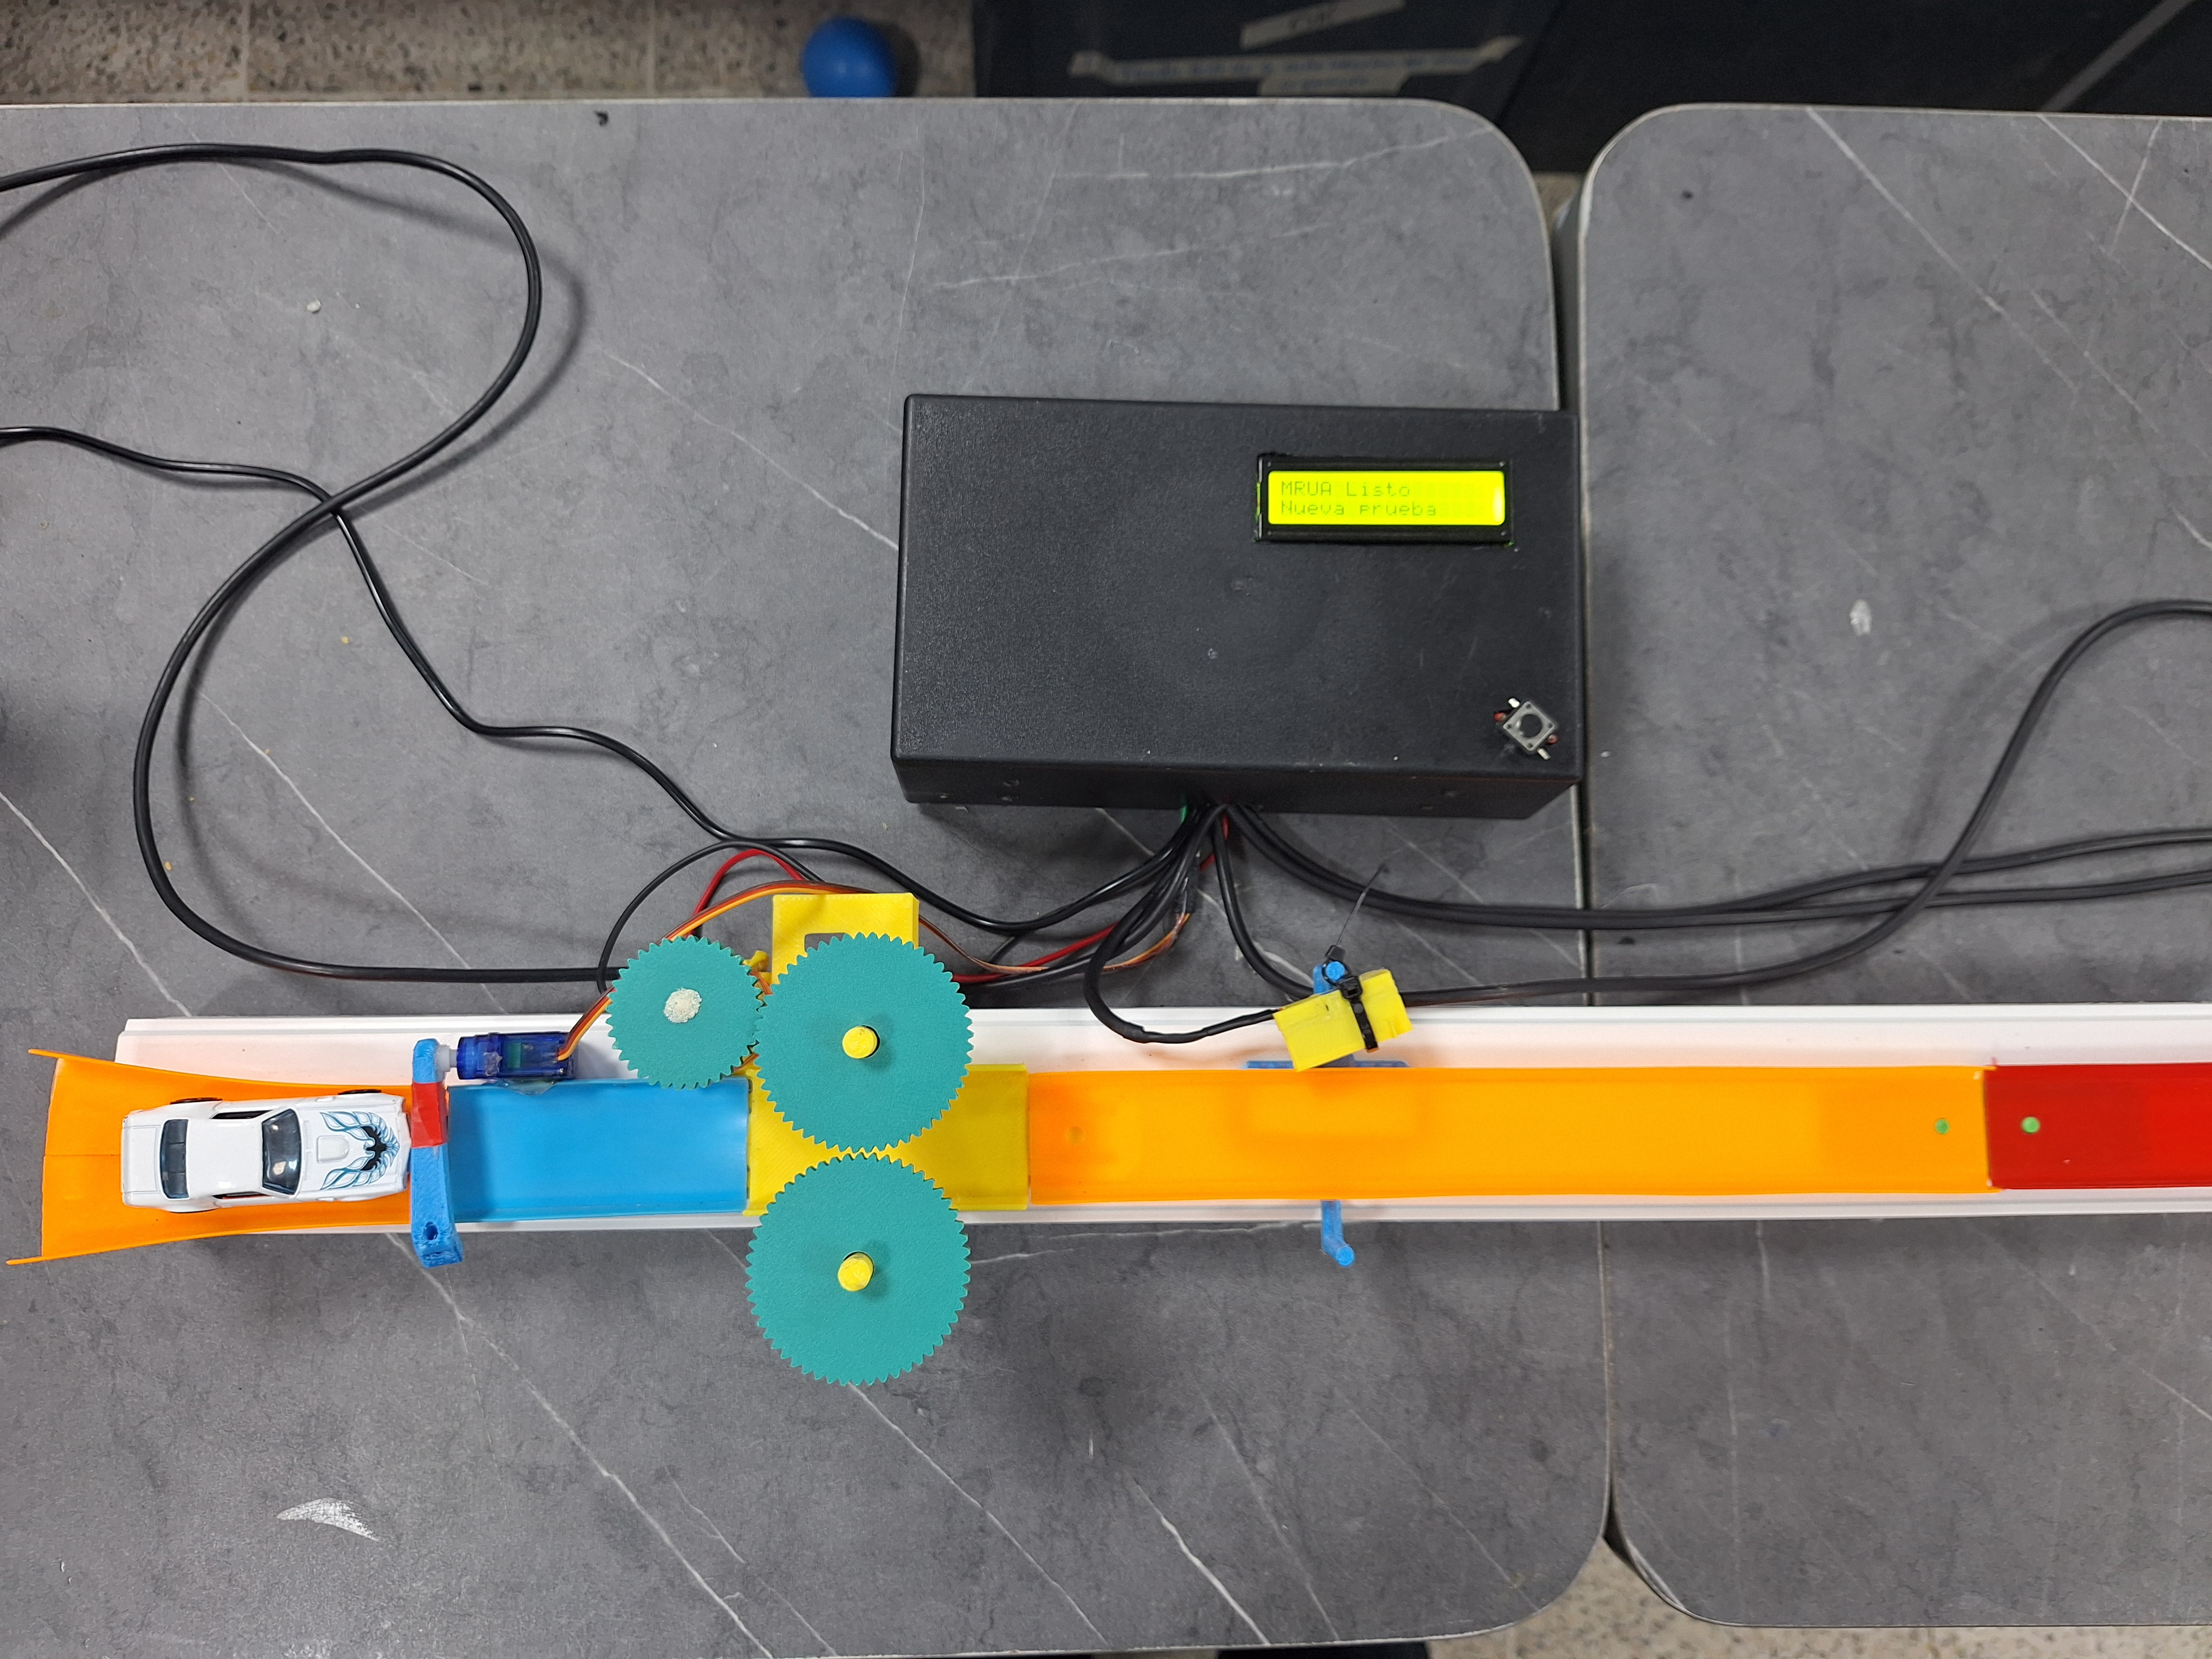
\includegraphics[width=0.45\textwidth]{figures/setup_overview_inicio.jpg}}
\hspace{0.5cm}
\subfloat[]{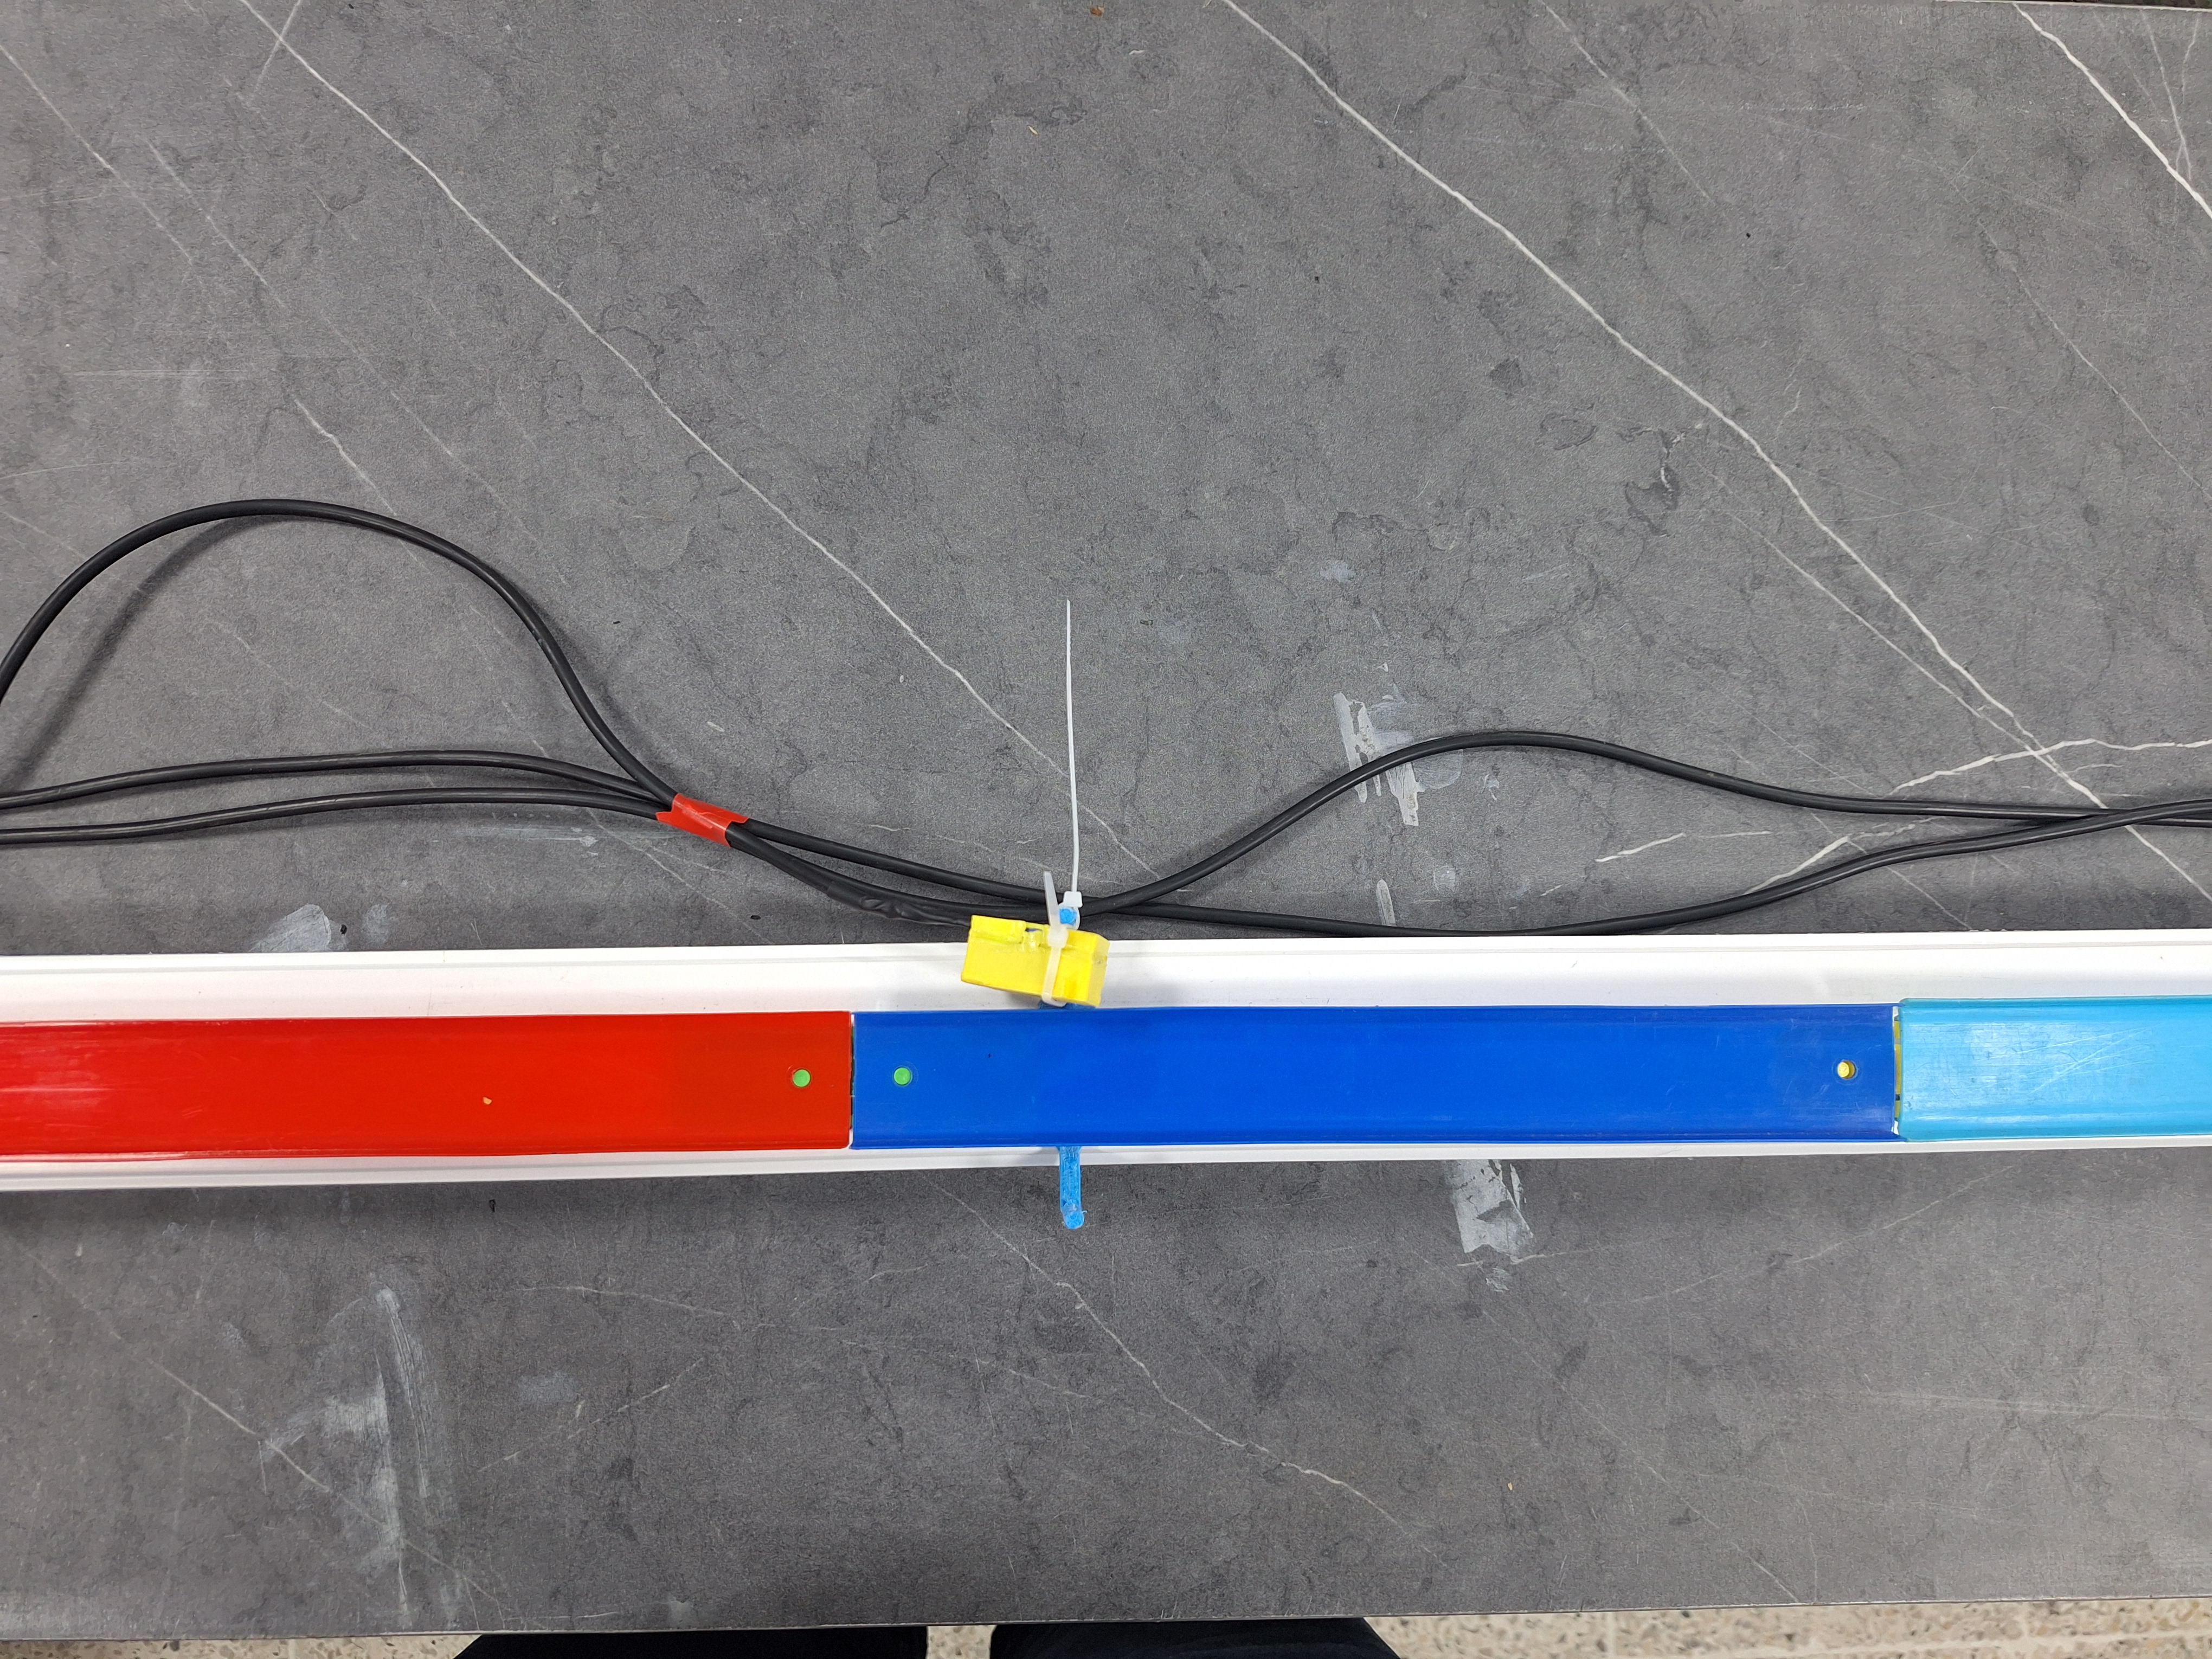
\includegraphics[width=0.45\textwidth]{figures/setup_overviewl_tramo2.jpg}}\\[0.3cm]
\subfloat[]{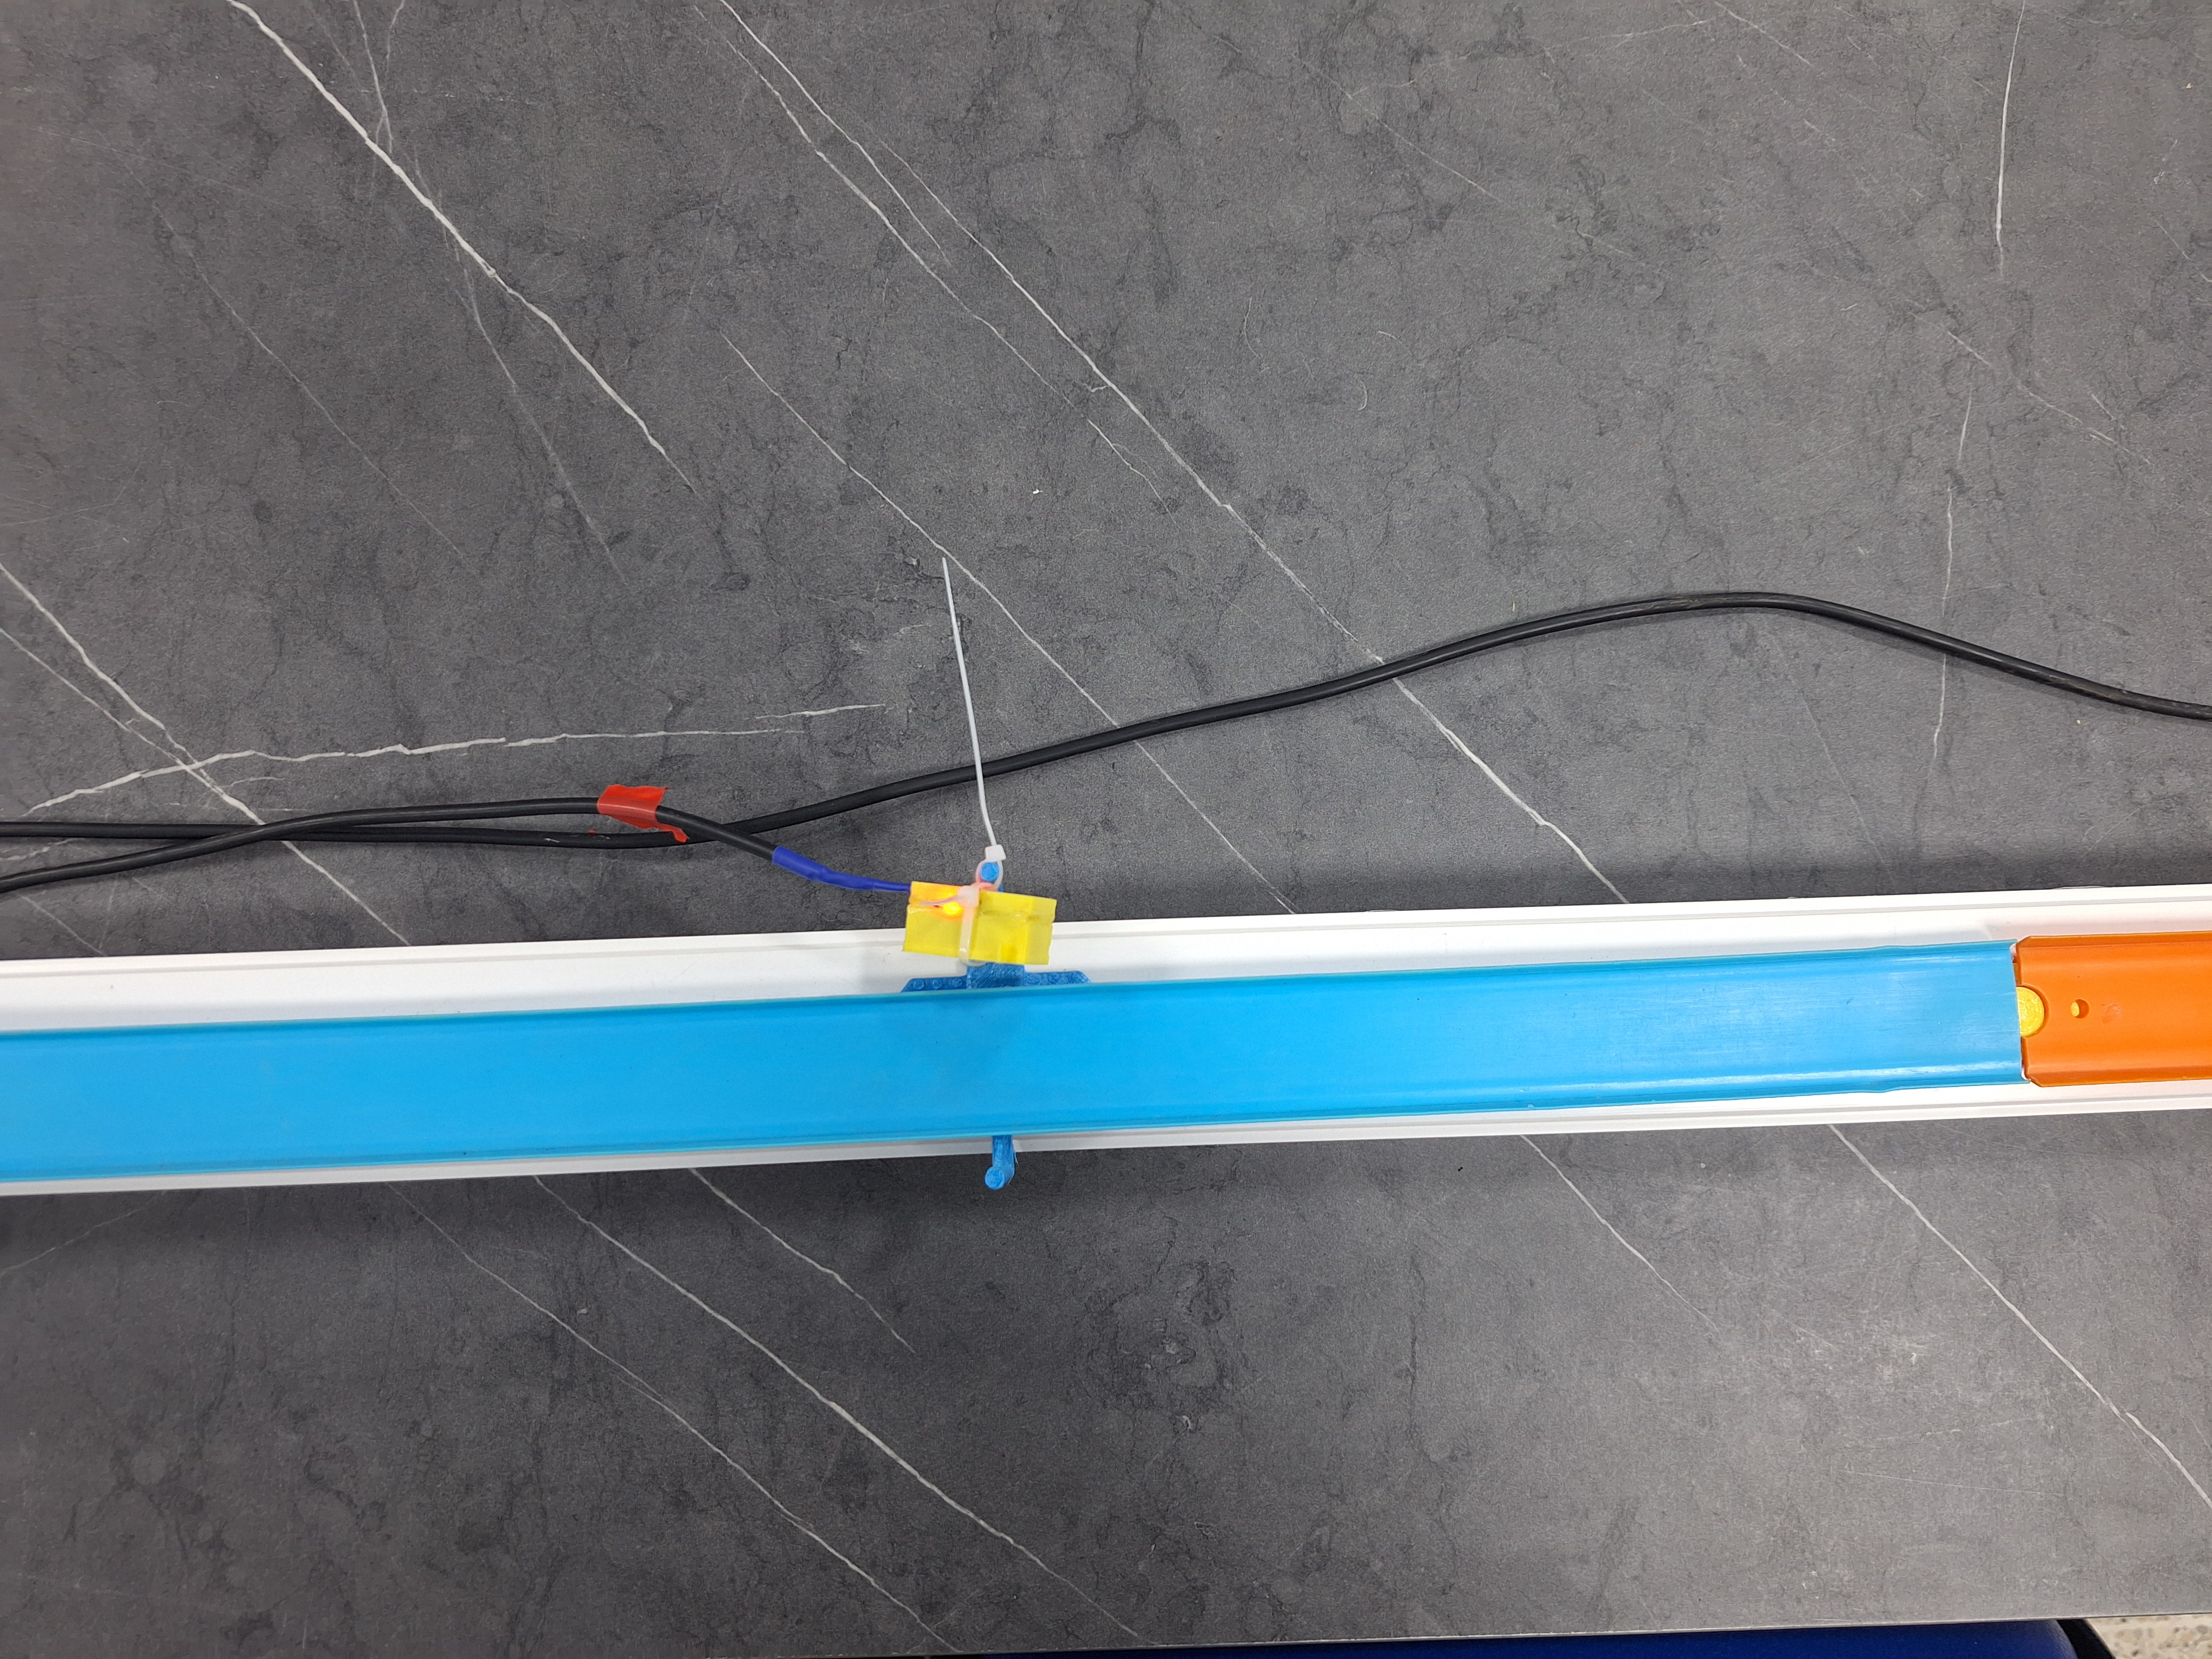
\includegraphics[width=0.45\textwidth]{figures/setup_overview_tramo3.jpg}}
\hspace{0.5cm}
\subfloat[]{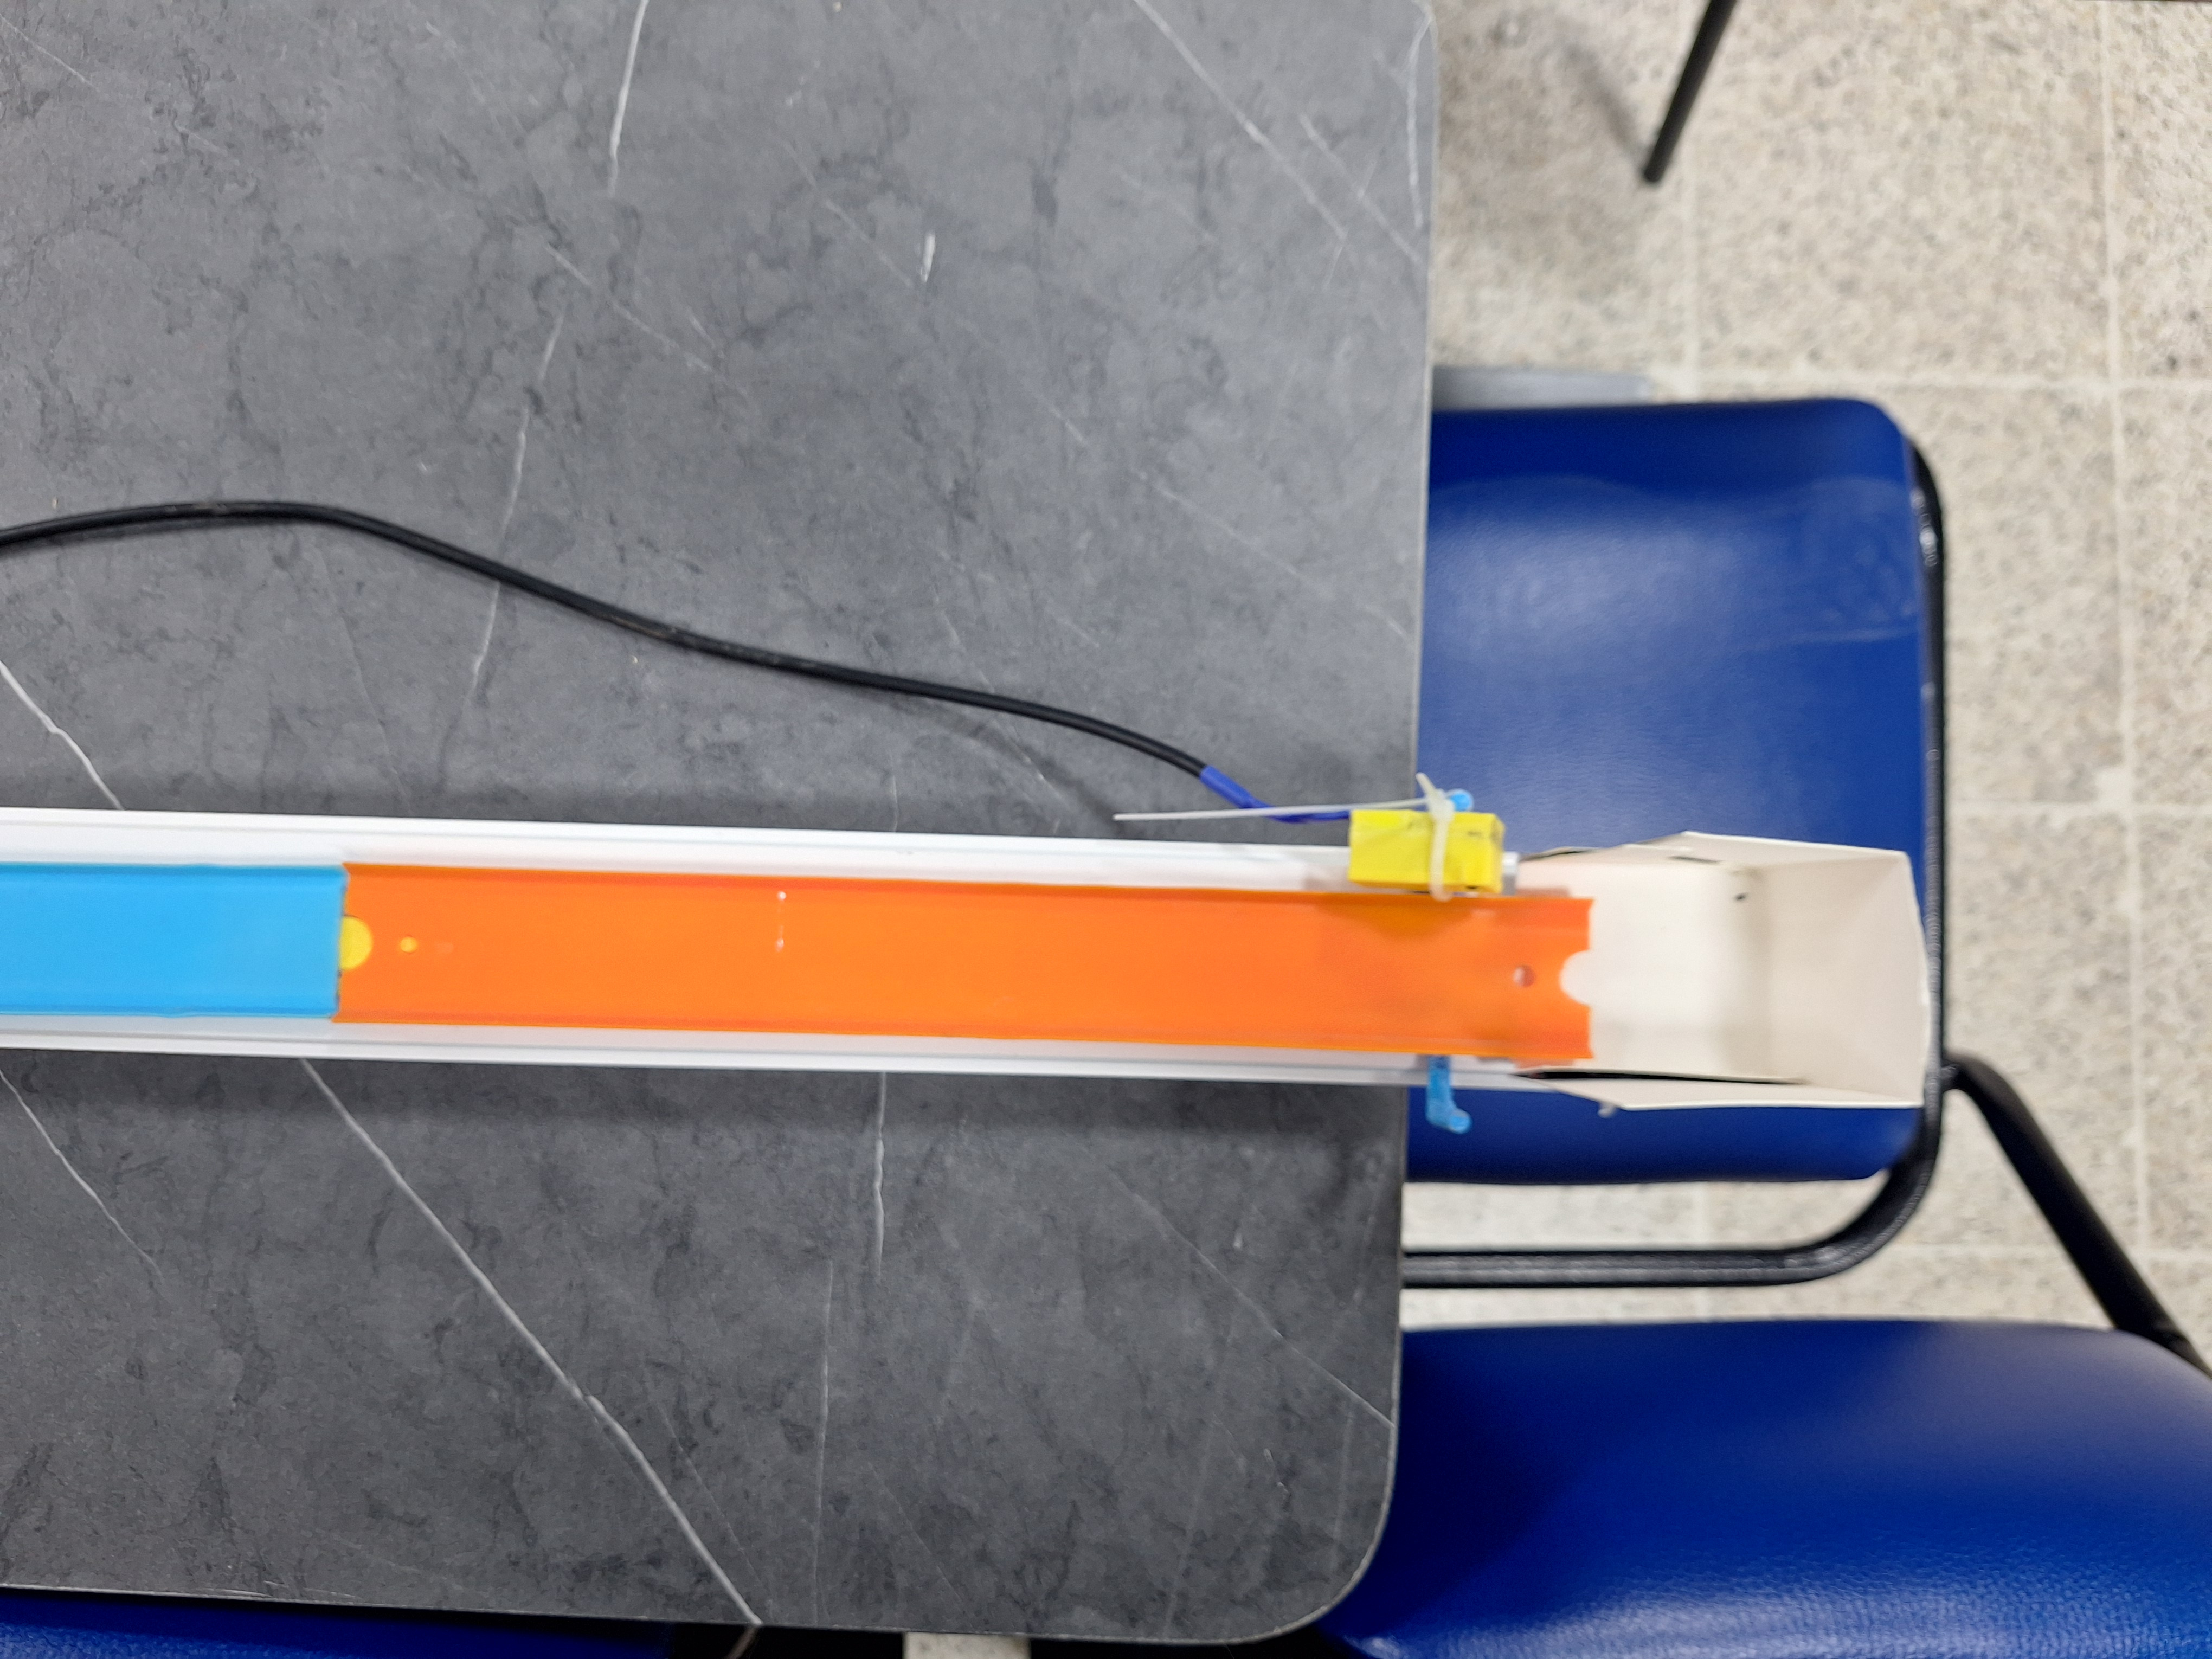
\includegraphics[width=0.45\textwidth]{figures/setup_overview_final.jpg}}
\caption{Detailed sections of the experimental setup: (a) start of the run; (b) section 2; (c) section 3; (d) endpoint and experiment completion.}
\label{fig:montaje_detalles}
\end{figure}

\begin{figure}[H]
\centering
\includegraphics[width=0.7\textwidth]{figures/setup_overview_completo.jpg}
\caption{General view of the IoT-based UARM experimental setup.}
\label{fig:vista_general}
\end{figure}

To facilitate remote interaction with the experiment, a web-based user interface was developed that centralizes system control and visualization. As shown in Figure~\ref{fig:interfaz_web}, this platform allows the user to start and stop the experimental sequence in a controlled manner. Additionally, the interface processes data in real time, automatically generating a graph with the kinematic results obtained after each trial. To ensure visual supervision of the process, a live video stream was integrated through a camera, enabling corroboration of the cart's physical movement with the received telemetric data.

\begin{figure}[H]
\centering
\includegraphics[width=0.7\textwidth]{figures/InterfazWeb.jpg}
\caption{Web interface developed for remote control and monitoring of the experiment.}
\label{fig:interfaz_web}
\end{figure}


\subsection{Sensor S1: Start of Motion}

Sensor S1 corresponds to the starting point of motion ($t = 0$). In both modalities, this sensor acts as the temporal trigger of the experiment; therefore, the recorded time is systematically zero or very close to zero.

\begin{table}[H]
	\caption{Statistical results for Sensor S1.}
	\label{tab:s1_results}
	\centering
	\small
	\begin{tabular}{lccc}
		\toprule
		\textbf{Modality} & \textbf{\(\bar{x}\) (s)} & \textbf{\(s\) (s)} & \textbf{\(n\)} \\
		\midrule
		In-Person & 0.00 & 0.00 & 35 \\
		Remote     & 0.00 & 0.00 & 35 \\
		\bottomrule
	\end{tabular}
\end{table}

\begin{figure}[H]
    \centering
    \includegraphics[width=0.7\textwidth]{figures/correlation_sensor_S1.png}
    \caption{Correlation plot for Sensor S1 (Remote vs. In-Person).}
    \label{fig:corr_s1}
\end{figure}

As shown in Figure~\ref{fig:corr_s1}, the data points are concentrated at the origin. The correlation coefficient is technically undefined or null (\(r \approx 0\)) because the data variance is zero (\(s=0\)). This behavior is physically expected and confirms that S1 functions correctly as a synchronization reference point for both the manual stopwatch and the digital control module. There are no fluctuations or experimental noise affecting this initial state.

\subsection{Sensor S2: First Intermediate Section}

Sensor S2 is located at the end of the first section of the track. The results in Table~\ref{tab:s2_results} show high consistency between the means of both modalities (1.17~s vs 1.19~s), with comparable standard deviations (0.15~s vs 0.16~s).

\begin{table}[H]
	\caption{Statistical results for Sensor S2.}
	\label{tab:s2_results}
	\centering
	\small
	\begin{tabular}{lccc}
		\toprule
		\textbf{Modalidad} & \textbf{\(\bar{x}\) (s)} & \textbf{\(s\) (s)} & \textbf{\(n\)} \\
		\midrule
		Presencial & 1.17 & 0.15 & 35 \\
		Remota     & 1.19 & 0.16 & 35 \\
		\bottomrule
	\end{tabular}
\end{table}

\begin{figure}[H]
    \centering
    \includegraphics[width=0.7\textwidth]{figures/correlation_sensor_S2.png}
    \caption{Correlation plot for Sensor S2 (Remote vs. In-Person).}
    \label{fig:corr_s2}
\end{figure}

Figure~\ref{fig:corr_s2} presents the scatter plot for S2, with a moderate Pearson correlation coefficient ($r = 0.61$, $R^2 = 0.37$, $N = 35$). This value reflects a statistically significant positive linear association between both modalities. The observed dispersion is consistent with the physical independence of the trials: since each pair (in-person, remote) corresponds to distinct physical events subject to different initial conditions of friction and cart release, a perfect correlation ($r \approx 1$) would be physically impossible. The value $r = 0.61$ with practically identical means ($\bar{x}_P = 1.17$~s vs.\ $\bar{y}_R = 1.19$~s, $\Delta\bar{x} = 0.02$~s) confirms that the IoT system captures the natural variability of UARM without introducing systematic bias.

\subsection{Sensor S3: Second Intermediate Section}

Sensor S3 captures the motion at a higher velocity. Table~\ref{tab:s3_results} shows very similar mean times for both modalities (1.66~s vs 1.69~s), with comparable standard deviations (0.23~s vs 0.24~s) indicating consistent measurement precision in both modes.

\begin{table}[H]
	\caption{Statistical results for Sensor S3.}
	\label{tab:s3_results}
	\centering
	\small
	\begin{tabular}{lccc}
		\toprule
		\textbf{Modalidad} & \textbf{\(\bar{x}\) (s)} & \textbf{\(s\) (s)} & \textbf{\(n\)} \\
		\midrule
		Presencial & 1.66 & 0.23 & 35 \\
		Remota     & 1.69 & 0.24 & 35 \\
		\bottomrule
	\end{tabular}
\end{table}

\begin{figure}[H]
    \centering
    \includegraphics[width=0.7\textwidth]{figures/correlation_sensor_S3.png}
    \caption{Correlation plot for Sensor S3 (Remote vs. In-Person).}
    \label{fig:corr_s3}
\end{figure}

Figure~\ref{fig:corr_s3} shows the scatter plot for S3, with $r = 0.62$, $R^2 = 0.39$, $N = 35$: the highest coefficient in the series, indicating a moderate positive correlation. This result is consistent with the sensor's larger temporal range ($\bar{x}_P = 1.66$~s), which amplifies the accumulated physical variability of UARM and enriches the statistical signal. The practically identical standard deviations ($\sigma_P = 0.23$~s vs.\ $\sigma_R = 0.24$~s, $\Delta\sigma = 0.01$~s) demonstrate that automated detection through hardware interrupts in the control module replicates the dispersion of manual timing with statistically equivalent fidelity.

\subsection{Sensor S4: End of Track}

Sensor S4 represents the final measurement point, where velocity is maximum. The results show excellent agreement between both modalities, with practically identical mean times (2.05~s vs 2.04~s) and comparable standard deviations (0.28~s vs 0.29~s). 
\begin{table}[H]
	\caption{Statistical results for Sensor S4.}
	\label{tab:s4_results}
	\centering
	\small
	\begin{tabular}{lccc}
		\toprule
		\textbf{Modalidad} & \textbf{\(\bar{x}\) (s)} & \textbf{\(s\) (s)} & \textbf{\(n\)} \\
		\midrule
		Presencial & 2.05 & 0.28 & 35 \\
		Remota     & 2.04 & 0.29 & 35 \\
		\bottomrule
	\end{tabular}
\end{table}

\begin{figure}[H]
    \centering
    \includegraphics[width=0.7\textwidth]{figures/correlation_sensor_S4.png}
    \caption{Correlation plot for Sensor S4 (Remote vs. In-Person).}
    \label{fig:corr_s4}
\end{figure}

The analysis of Figure~\ref{fig:corr_s4} confirms the pattern observed in the previous sensors. Both in-person and remote measurements show comparable dispersion ($s=0.28$~s and $s=0.29$~s respectively), with practically identical mean times (2.05~s vs 2.04~s). The correlation coefficient is consistent with the independence of trials; each measurement captures the natural variability of the UARM phenomenon under different initial conditions ($r = 0.61$, $R^2 = 0.38$, $N = 35$). The agreement between both modalities demonstrates that the IoT retrofitting system successfully replicates the measurement capabilities of the traditional configuration, providing reliable kinematic data suitable for quantitative analysis of uniformly accelerated motion.

%- - - - - - - - - - - - - - - - - - - - - -
\subsection{Global Kinematic Analysis and Stability}

Figure~\ref{fig:vel_profile} shows the average velocity profile as a function of position for both modalities, calculated with Equation~\ref{eq:velocidad}. The remote and in-person modality curves are practically indistinguishable across the three track segments, with comparable error bars, evidencing that the IoT system captures the UARM evolution with fidelity equivalent to the in-person setup.
\begin{figure}[H]
  \centering
  \includegraphics[width=0.80\linewidth]{figures/velocity_profile.png}
  \caption{Average velocity profile vs. mean segment position for the remote (blue, circles) and in-person (red, squares) modalities. Error bars represent $\pm 1\sigma$. The overlap of both curves confirms the kinematic equivalence of the proposed system.}
  \label{fig:vel_profile}
\end{figure}

Figure~\ref{fig:accel_box} presents the distribution of estimated experimental acceleration using Equation~\ref{eq:aceleracion} for the 35 trials of each modality. Both distributions exhibit comparable medians and interquartile ranges, with identical means ($\mu = 0.98$~m/s$^2$ for both modalities) and similar standard deviations ($\sigma = 0.26$~m/s$^2$ remote vs. $\sigma = 0.28$~m/s$^2$ in-person). This result constitutes the strongest evidence of the system's technical equivalence: IoT instrumentation and manual timing produce statistically indistinguishable estimates of the experiment's central physical quantity.
\begin{figure}[H]
  \centering
  \includegraphics[width=0.75\linewidth]{figures/acceleration_boxplot.png}
  \caption{Distribution of estimated experimental acceleration for the remote ($\mu = 0.98$~m/s$^2$, $\sigma = 0.26$~m/s$^2$) and in-person ($\mu = 0.98$~m/s$^2$, $\sigma = 0.28$~m/s$^2$) modalities. Box plots show median, interquartile range, and extreme values for $n = 35$ trials per modality.}
  \label{fig:accel_box}
\end{figure}

Figure~\ref{fig:mrua_teorico} compares the experimental position vs. time data with the theoretical UARM model defined by Equation~\ref{eq:mruateorico}. The theoretical model ($a \approx 0.92$~m/s$^2$) was calculated from the measured track inclination angle. The experimental points from both modalities are situated in the vicinity of the theoretical curve, with horizontal error bars reflecting the temporal dispersion at each sensor. The mean experimental acceleration ($\mu = 0.98$~m/s$^2$) slightly exceeds the theoretical value by 6.5\%, a difference attributable to imprecisions in the measurement of angle $\theta$ and rotational inertia effects of the cart not considered in the simplified model.
The 6.5\% difference between the experimental value
($\mu = 0.98$~m/s$^2$) and the theoretical value
($a_{\text{theoretical}} \approx 0.92$~m/s$^2$) falls
within the expected margin for this type of setup.
The theoretical model of Equation~\ref{eq:mruateorico}
assumes zero friction and inclination angle measured with
a conventional measuring tape; the residual cart friction
and angular uncertainty introduce a systematic deviation
of this magnitude, which is consistent with values
reported in similar works~\cite{r10}.
\begin{figure}[H]
  \centering
  \includegraphics[width=0.80\linewidth]{figures/experimental_vs_theoretical_mrua.png}
  \caption{Position vs. time: comparison between the theoretical UARM model ($a \approx 0.92$~m/s$^2$, gray dashed line) and experimental data from the remote (blue circles) and in-person (red squares) modalities. Horizontal error bars represent $\pm 1\sigma$ of detection times at each sensor.}
  \label{fig:mrua_teorico}
\end{figure}

Figure~\ref{fig:stability} shows the successful event capture rate for both modalities. The in-person modality achieved 100\% capture in all trials, while the remote modality recorded a rate of 98.5\%, corresponding to the loss of 1 detection event in the 2,380 total MQTT transmissions generated during the 35 trials (4 sensors $\times$ 17 segments). This 1.5 percentage point difference is attributable to a momentary WiFi network disconnection documented during the session, and not to a systematic limitation of the implemented MQTT protocol.
\begin{figure}[H]
  \centering
  \includegraphics[width=0.65\linewidth]{figures/stability_success_rate.png}
  \caption{Successful event capture rate for the remote (98.5\%) and in-person (100.0\%) modalities. The 1.5 percentage point difference is attributable to a transient WiFi disconnection during a testing session.}
  \label{fig:stability}
\end{figure}

%-------------------------------------------------
% DISCUSION
%-------------------------------------------------

\section{Discussion}

\subsection{Interpretation of Temporal and Kinematic Results}

The results obtained demonstrate that the IoT retrofitting system is capable of capturing the dynamics of the UARM experiment with fidelity comparable to and even superior in stability to the traditional in-person setup. Contrary to expectations for distributed systems, measurements in the remote modality presented controlled dispersion, evidencing the efficiency of interrupt handling in the control module. Data consistency suggests that network latency, although present, did not degrade the quality of kinematic data collection thanks to local timestamping.

\subsection{Implications for IoT-Based Retrofitting of Physics Laboratories}

The technical viability of the proposed model has direct implications for the modernization of educational infrastructures with limited resources. The retrofitting approach demonstrates that it is possible to transform classic equipment into connected digital assets without the need to replace the original instrumentation. The modular architecture adopted enables efficient scalability, where the sensing and control layer is decoupled from visualization and storage services. The results validate that low-cost solutions based on mass-market hardware can achieve precision levels adequate for academic purposes, facilitating the transition toward hybrid learning environments that do not depend exclusively on physical presence in the laboratory.

It is important to highlight that the obtained Pearson correlation coefficients ($r = 0.61$--$0.62$) should not be interpreted as a limitation of the IoT system. The values of $r = 0.61$--$0.62$ are consistent with what is expected for independent unpaired series sharing the same source of physical variability: the stochastic nature of the manual cart launch introduces identical dispersion in both modalities, which limits the correlation coefficient without affecting the equivalence of distributions~\cite{giavarina2015}. The Bland--Altman analysis (Table~\ref{tab:bland_altman}) confirms that the 95\% limits of agreement are below 0.08~s, which is technically acceptable for the pedagogical purpose of the experiment.

\begin{table}[H]
\caption{Systematic comparison with related works.}
\label{tab:comparacion}
\small
\begin{adjustwidth}{-\extralength}{0cm}
	\renewcommand{\arraystretch}{1.4}
	\begin{tabular}{p{3.2cm}p{2.0cm}p{2.2cm}p{3.2cm}p{1.4cm}p{1.6cm}p{1.2cm}p{1.2cm}}
		\toprule
		\textbf{Study} & \textbf{Strategy} & \textbf{Hardware} & \textbf{Remote vs.\ in-person validation} & \textbf{Cost (USD)} & \textbf{Limited resources} & \textbf{Native web} & \textbf{Open source} \\
		\midrule
		This work                               & Retrofitting   & ESP32 + RPi~4   & Yes (quantitative) & $<$150      & Yes    & S\'i    & S\'i    \\
		Lustig \textit{et al.}~\cite{r10}          & Retrofitting   & ESP32 + RPi     & No                  & $\sim$200   & Partial & S\'i    & S\'i    \\
		P\'erez-Cham\'e \textit{et al.}~\cite{r11} & New hardware & ESP32           & No                  & $\sim$100   & S\'i    & No      & Parcial \\
		Guerrero-Osuna \textit{et al.}~\cite{r4}   & New system  & Arduino + cloud & No                  & $>$500      & No      & S\'i    & No      \\
		Viswanadh \textit{et al.}~\cite{r2}        & Retrofitting   & RPi + sensors  & No                  & $\sim$200   & S\'i    & Parcial & No      \\
		Fuertes \textit{et al.}~\cite{r3}          & New system  & Embedded + cloud & No                  & $>$500      & No      & S\'i    & No      \\
		\bottomrule
	\end{tabular}
\end{adjustwidth}
\end{table}


\subsection{Comparison with Related Works}

When contrasting the results with prior literature, fundamental similarities are observed with the works of Viswanadh \textit{et al.}~\cite{r2} and Lustig \textit{et al.}~\cite{r5} regarding the effectiveness of modular architectures for remote experiments. However, the present study contributes a specific quantitative validation for the case of UARM, extending the proposals of Guerrero-Osuna \textit{et al.}~\cite{r4} and Fuertes \textit{et al.}~\cite{r3}, who focused primarily on motor control. Unlike the SmartIPL-based solutions reviewed by Zhao~\cite{r6}, which depend on smartphone internal sensors, the implemented system offers a fixed and dedicated infrastructure that ensures greater repeatability in test conditions while maintaining the economic accessibility of the setup.

\subsection{Limitations of the Study}

Despite the satisfactory performance of the prototype, intrinsic limitations in the scope of the research are identified. First, although stability was high, the system still depends on the continuous availability of the MQTT server for real-time data transmission. Second, the number of trials conducted (n=35 per modality), although robust, is limited to a controlled university laboratory environment. Additionally, the experiment is conducted under mechanical conditions where factors such as residual cart friction and micrometric alignment of optical sensors introduce physical variations that are independent of the IoT instrumentation.

\subsection{Future Work}

Future research lines are oriented toward the optimization of the perception layer and system robustness. The integration of sensors with higher temporal resolution and the use of communication protocols with traffic prioritization to minimize the impact of network latency are proposed. Likewise, it is pertinent to increase the volume of trials to strengthen the statistical analysis and perform explicit latency measurements at each stage of the data chain. From a functional perspective, the system can be expanded to instrument other dynamics and energy experiments, integrating data flows with educational learning management platforms (LMS) to automate the evaluation of experimental practices.

\section{Conclusions}

The proposed IoT retrofitting system demonstrated the ability to reproduce UARM measurements with statistical precision equivalent to the in-person reference setup. Mean differences between modalities were below 0.03~s at all four measurement points, with $\Delta\sigma < 0.02$~s across all sensors (Table~\ref{tab:resumen_global}). The most significant result is the equality of mean experimental acceleration in both modalities ($\mu = 0.98$~m/s$^2$, $n = 35$ each), with a 6.5\% deviation from the expected theoretical value ($a \approx 0.92$~m/s$^2$), attributable to setup imprecisions rather than the IoT measurement system (Figure~\ref{fig:accel_box}). The successful event capture rate was 98.5\% in remote mode, with a single documented event loss across the 2,380 MQTT transmissions executed.

The central contribution of this work is the quantitative validation, through Pearson correlation metrics ($r = 0.61$--$0.62$), velocity profiles, and acceleration distributions, that a low-cost IoT system ($<$~USD~150) based on Edge computing technology (ESP32) can replicate the measurement capabilities of an in-person kinematics physics setup. The proposed three-layer architecture, with open-source code available on GitHub (RemotePhysicsLab~\cite{r15}), is directly replicable and adaptable to other experiments and resource-limited institutional contexts.

The study presents three main limitations: (1)~validation is limited to a single kinematics experiment (UARM) in a specific institutional environment (PUCE Esmeraldas); (2)~learning indicators and usability perception with real students were not evaluated; (3)~system stability is conditioned by the availability and quality of the laboratory's WiFi network.

The priority lines of future research are:
\begin{enumerate}[label=(\arabic*)]
  \item Extension of the platform to other physics experiments: dynamics, conservation of energy, and wave experiments.
  \item Learning assessment with real student groups, comparing results in remote vs. in-person modalities.
  \item Integration with LMS systems (Moodle, Canvas) for automatic evaluation of laboratory practices.
  \item Incorporation of sensors with higher temporal resolution (photogates $<$~1~ms) for higher-speed experiments.
  \item Implementation of MQTT QoS level~1 and automatic reconnection protocol for environments with unstable networks.
\end{enumerate}

%-------------------------------------------------
% REFERENCIAS
%-------------------------------------------------

\reftitle{References}
\begin{thebibliography}{999}

\bibitem{r1}
Lahme, S.Z.; Klein, P.; Lehtinen, A.; M\"uller, A.; Pirinen, P.; Ron\v{c}evi\'c, L.; Su\v{s}ac, A.
Physics lab courses under digital transformation: A trinational survey among university lab instructors about the role of new digital technologies and learning objectives.
\textit{Phys. Rev. Phys. Educ. Res.} \textbf{2023}, \textit{19}, 020159.
\href{https://doi.org/10.1103/PhysRevPhysEducRes.19.020159}{https://doi.org/10.1103/PhysRevPhysEducRes.19.020159}.

\bibitem{r2}
Viswanadh, K.S.; Gureja, A.; Walchatwar, N.; Agrawal, R.; Sinha, S.; Chaudhari, S.; Vaidhyanathan, K.; Hussain, A.M.
Engineering End-to-End Remote Labs Using IoT-Based Retrofitting.
\textit{IEEE Access} \textbf{2024}, \textit{PP}, 1--1.
\href{https://doi.org/10.1109/ACCESS.2024.3523066}{https://doi.org/10.1109/ACCESS.2024.3523066}.

\bibitem{r3}
Fuertes, J.J.; Mart\'inez, J.M.; Dormido, S.; Vargas, H.; S\'anchez, J.; Duro, N.
Virtual and Remote Laboratory of a DC Motor for Learning Control Theory.
\textit{Int. J. Eng. Educ.} \textbf{2011}, \textit{27}, 1--12.

\bibitem{r4}
Guerrero-Osuna, H.A.; Garc\'ia-V\'azquez, F.A.; Ibarra-Delgado, S.; Sol\'is-S\'anchez, L.O.
Developing a Cloud and IoT-Integrated Remote Laboratory to Enhance Education 4.0: An Approach for FPGA-Based Motor Control.
\textit{Appl. Sci.} \textbf{2024}, \textit{14}, 10115.

\bibitem{r5}
Lustig, F.; Kuri\v{s}\v{c}\'ak, P.; Brom, P.; Dvo\v{r}\'ak, J.
Open Modular Hardware and Software Kit for Creations of Remote Experiments Accessible from PC and Mobile Devices.
\textit{Int. J. Online Eng. (iJOE)} \textbf{2016}, \textit{12}, 30--36.
\href{https://doi.org/10.3991/ijoe.v12i07.5833}{https://doi.org/10.3991/ijoe.v12i07.5833}.

\bibitem{r6}
Zhao, Y.
Smartphone-Based Undergraduate Physics Labs: A Comprehensive Review.
\textit{IEEE Access} \textbf{2024}, \textit{13}, 1106--1132.
\href{https://doi.org/10.1109/ACCESS.2024.3523066}{https://doi.org/10.1109/ACCESS.2024.3523066}.

\bibitem{r7}
Dizdarevic, J.; Jukan, A.
Engineering an IoT--Edge--Cloud Computing System Architecture: Lessons Learnt from an Undergraduate Laboratory Course.
\textit{IoT} \textbf{2022}, \textit{3}, 145--163.
\href{https://doi.org/10.3390/iot3010010}{https://doi.org/10.3390/iot3010010}.

\bibitem{r8}
Azad, A.K.M.
Use of Internet of Things for Remote Laboratory Settings.
\textit{IoT} \textbf{2021}, \textit{2}, 203--232.
\href{https://doi.org/10.3390/iot2020011}{https://doi.org/10.3390/iot2020011}.

\bibitem{r9}
Palmer, C.; Roullier, B.; Aamir, M.; McQuade, F.; Stella, L.; Anjum, A.
Digital Twinning Remote Laboratories for Online Practical Learning.
\textit{Sensors} \textbf{2022}, \textit{22}, 2351.
\href{https://doi.org/10.3390/s22062351}{https://doi.org/10.3390/s22062351}.

\bibitem{r10}
Lustig, A.; Biard, V. \textit{et al.}
Engineering End-to-End Remote Labs using IoT-based Retrofitting.
\textit{arXiv} \textbf{2024}, arXiv:2402.05466.
Available online: \url{https://arxiv.org/abs/2402.05466} (accessed on 5 December 2025).

\bibitem{r11}
P\'erez-Cham\'e, J.H. \textit{et al.}
Development of an educational low-cost and ESP32-based platform for fundamental physics experiments.
\textit{Comput. Appl. Eng. Educ.} \textbf{2023}.
\href{https://doi.org/10.1002/cae.22674}{https://doi.org/10.1002/cae.22674}.

\bibitem{r12}
Marosan, A. \textit{et al.}
Real-time data acquisition with ESP32 for IoT applications in educational environments.
\textit{Int. Conf. Appl. Math. Sci. (ICMAS)} \textbf{2024}, \textit{19}(2), 61--68.
Available online: \url{http://www.icmas.eu/Journal_archive_files/Vol_19-Issue2_2024_PDF/61-68_MAROSAN.pdf} (accessed on 5 December 2025).

\bibitem{r13}
Idoyaga, I. \textit{et al.}
The Use of Remote Laboratories in University Physics: Challenges and Opportunities in Latin America.
In \textit{Proceedings of the Symposium ICASE-MIDEC GIREP 2023}.
Available online: \url{https://indico.cern.ch/event/1175859/} (accessed on 5 December 2025).

\bibitem{r14}
Vera, M. \textit{et al.}
An\'alisis comparativo de la ense\~nanza de la f\'isica en universidades latinoamericanas durante la pandemia COVID-19.
\textit{Rev. Invecom} \textbf{2025}.
Available online: \url{https://revistainvecom.org/index.php/invecom/article/view/4234} (accessed on 5 December 2025).

\bibitem{r15}
Sosa Mej\'ia, W.S.
\textit{RemotePhysicsLab: Prototipo de laboratorio de f\'isica h\'ibrido basado en IoT}.
Repositorio GitHub.
Available online: \url{https://github.com/waltersosa/RemotePhysicsLab.git} (accessed on 5 December 2025).

\bibitem{r16}
Hevner, A.R.; March, S.T.; Park, J.; Ram, S.
Design Science in Information Systems Research.
\textit{MIS Q.} \textbf{2004}, \textit{28}, 75--105.

\bibitem{r17}
ISO/IEC.
\textit{ISO/IEC 15288:2015 Systems and Software Engineering---System Life Cycle Processes};
International Organization for Standardization: Geneva, Switzerland, 2015.

\bibitem{r18}
Mattel, Inc.
\textit{Hot Wheels Track Sets}.
Available online: \url{https://shop.mattel.com/pages/hot-wheels} (accessed on 5 December 2025).

\bibitem{r19}
Mattel, Inc.
\textit{Hot Wheels Cars}.
Available online: \url{https://shop.mattel.com/collections/hot-wheels-cars} (accessed on 5 December 2025).

\bibitem{r20}
Vishay Intertechnology, Inc.
\textit{TCRT5000 Reflective Optical Sensor}.
Available online: \url{https://www.vishay.com/docs/83751/tcrt5000.pdf} (accessed on 5 December 2025).

\bibitem{r21}
Espressif Systems.
\textit{ESP32-WROOM-32 Datasheet}.
Available online: \url{https://www.espressif.com/sites/default/files/documentation/esp32-wroom-32_datasheet_en.pdf} (accessed on 5 December 2025).

\bibitem{r22}
Thingiverse.
\textit{Mechanical Support for Track-Based Experiments} (Thing 3630616).
Available online: \url{https://www.thingiverse.com/thing:3630616} (accessed on 5 December 2025).

\bibitem{r23}
Thingiverse.
\textit{3D Printed Modular Track Components} (Thing 3485484).
Available online: \url{https://www.thingiverse.com/thing:3485484} (accessed on 5 December 2025).

\bibitem{r24}
Thingiverse.
\textit{3D Printed Structural Reinforcement Parts} (Thing 4381935).
Available online: \url{https://www.thingiverse.com/thing:4381935} (accessed on 5 December 2025).

\bibitem{r25}
Thingiverse.
\textit{3D Printed Mechanical Pusher Mechanism} (Thing 2806324).
Available online: \url{https://www.thingiverse.com/thing:2806324} (accessed on 5 December 2025).

\bibitem{r26}
Tower Pro.
\textit{SG90 Micro Servo Motor Datasheet}.
Available online: \url{http://www.ee.ic.ac.uk/pjs99/projects/servo/sg90_datasheet.pdf} (accessed on 5 December 2025).

\bibitem{r27}
Stepperonline.
\textit{NEMA 17 Stepper Motor Bipolar Datasheet}.
Available online: \url{https://www.omc-stepperonline.com/download/17HS19-2004S1.pdf} (accessed on 5 December 2025).

\bibitem{r28}
STMicroelectronics.
\textit{L298N Dual H-Bridge Motor Driver Datasheet}.
Available online: \url{https://www.st.com/resource/en/datasheet/l298.pdf} (accessed on 5 December 2025).

\bibitem{r29}
Generic Electronics Suppliers.
\textit{LCD 20x4 Display with I2C Interface Datasheet}.
Available online: \url{https://www.sparkfun.com/datasheets/LCD/HD44780.pdf} (accessed on 5 December 2025).

\bibitem{r30}
Generic Electronics Suppliers.
\textit{Tactile Push Button Switch for Breadboard}.
Available online: \url{https://www.adafruit.com/product/367} (accessed on 5 December 2025).

\bibitem{r31}
USB Implementers Forum.
\textit{USB Type-C Cable Specification}.
Available online: \url{https://www.usb.org/sites/default/files/USB\%20Type-C\%20Spec\%20R2.0\%20-\%20August\%202019.pdf} (accessed on 5 December 2025).

\bibitem{r32}
IEEE.
\textit{IEEE Standard for Wireless LAN Medium Access Control (MAC) and Physical Layer (PHY) Specifications}.
Available online: \url{https://ieeexplore.ieee.org/document/9363693} (accessed on 5 December 2025).

\bibitem{r33}
Generic Electronics Suppliers.
\textit{Dupont Jumper Wires (Male-Female and Female-Female)}.
Available online: \url{https://www.adafruit.com/category/289} (accessed on 5 December 2025).

\bibitem{r34}
Generic Electronics Suppliers.
\textit{Plastic Project Enclosure Box (135x75x40 mm)}.
Available online: \url{https://www.digikey.com/en/products/filter/enclosures/287} (accessed on 5 December 2025).

\bibitem{r35}
Generic Electronics Suppliers.
\textit{AC-DC Power Adapter 12V/1A}.
Available online: \url{https://www.digikey.com/en/products/filter/power-supplies-external-internal-off-board/171} (accessed on 5 December 2025).

\bibitem{r36}
Insta360.
\textit{Insta360 Link---4K AI Webcam Technical Specifications}.
Available online: \url{https://onlinemanual.insta360.com/link/en-us/introduction} (accessed on 5 December 2025).

\bibitem{r37}
Raspberry Pi Ltd.
\textit{Raspberry Pi 4 Model B Product Brief}.
Available online: \url{https://datasheets.raspberrypi.com/rpi4/raspberry-pi-4-product-brief.pdf} (accessed on 5 December 2025).

\bibitem{r38}
EMQ Technologies Co., Ltd.
\textit{EMQX---MQTT Platform for IoT Data Streaming Documentation}.
Available online: \url{https://docs.emqx.com/en/emqx/v5.0/} (accessed on 5 December 2025).

\bibitem{r39}
EMQ Technologies Co., Ltd.
\textit{MQTTX: Your All-in-One MQTT Client Toolbox Documentation}.
Available online: \url{https://mqttx.app/docs} (accessed on 5 December 2025).

\bibitem{r40}
OpenJS Foundation.
\textit{Node.js API Documentation}.
Available online: \url{https://nodejs.org/api/} (accessed on 5 December 2025).

\bibitem{r41}
OpenJS Foundation.
\textit{Express API Reference}.
Available online: \url{https://expressjs.com/en/4x/api.html} (accessed on 5 December 2025).

\bibitem{r42}
MongoDB, Inc.
\textit{MongoDB Documentation}.
Available online: \url{https://www.mongodb.com/docs/manual/} (accessed on 5 December 2025).

\bibitem{r43}
Mongoose.
\textit{Mongoose ODM API Documentation}.
Available online: \url{https://mongoosejs.com/docs/api.html} (accessed on 5 December 2025).

\bibitem{r44}
Vercel, Inc.
\textit{Next.js Documentation}.
Available online: \url{https://nextjs.org/docs} (accessed on 5 December 2025).

\bibitem{r45}
Meta Platforms, Inc.
\textit{React Reference Documentation}.
Available online: \url{https://react.dev/reference/react} (accessed on 5 December 2025).

\bibitem{r46}
Arduino AG.
\textit{Arduino IDE 2.x Documentation}.
Available online: \url{https://www.arduino.cc/en/software} (accessed on 5 December 2025).

\bibitem{r47}
Python Software Foundation.
\textit{Python 3 Documentation}.
Available online: \url{https://docs.python.org/3/} (accessed on 5 December 2025).

\bibitem{r48}
Atzori, L.; Iera, A.; Morabito, G.
The Internet of Things: A survey.
\textit{Comput. Netw.} \textbf{2010}, \textit{54}, 2787--2805.
\href{https://doi.org/10.1016/j.comnet.2010.05.010}{https://doi.org/10.1016/j.comnet.2010.05.010}.

\bibitem{r49}
Eraser Labs, Inc.
\textit{Eraser---AI Co-Pilot for Technical Design and Documentation}.
Available online: \url{https://www.eraser.io} (accessed on 5 December 2025).

\bibitem{r50}
OpenAI. \textit{ChatGPT}.
Available online: \url{https://chat.openai.com} (accessed on 23 January 2026). Content generated with the assistance of ChatGPT.

\bibitem{r51}
Hern\'andez, R. \textit{et al.}
Remote Laboratory for developing IoT systems in engineering education.
In \textit{Proceedings of the ACM Technical Symposium on Computer Science Education}; ACM: New York, NY, USA, \textbf{2025}.
\href{https://doi.org/10.1145/3716554.3716602}{https://doi.org/10.1145/3716554.3716602}.

\bibitem{r52}
Chang, H.Y. \textit{et al.}
Deploying an IoT-based remote physics lab platform to support undergraduate mechanics education.
\textit{Phys. Educ.} \textbf{2024}, \textit{59}, 065012.

\bibitem{r53}
Kaur, G. \textit{et al.}
Design and Implementation of ESP32-Based IoT Devices for Real-Time Monitoring Applications.
\textit{Sensors} \textbf{2023}, \textit{23}, 6437.
\href{https://doi.org/10.3390/s23156437}{https://doi.org/10.3390/s23156437}.


\bibitem{bland1986}
Bland, J.M.; Altman, D.G.
Statistical methods for assessing agreement between two methods of clinical measurement.
\textit{The Lancet} \textbf{1986}, \textit{327}(8476), 307--310.
\href{https://doi.org/10.1016/S0140-6736(86)90837-8}{doi:10.1016/S0140-6736(86)90837-8}

\bibitem{giavarina2015}
Giavarina, D.
Understanding Bland Altman analysis.
\textit{Biochemia Medica} \textbf{2015}, \textit{25}(2), 141--151.
\href{https://doi.org/10.11613/BM.2015.015}{doi:10.11613/BM.2015.015}

\end{thebibliography}


\end{document}